\documentclass[11pt,a4paper]{article}

\usepackage[utf8]{inputenc}
\usepackage[english]{babel}
\usepackage[left=2cm,right=2cm,top=2cm,bottom=2cm]{geometry}

\usepackage{csquotes}
\usepackage{graphicx}
\graphicspath{ {./figs} }

\usepackage{caption}
\usepackage{subcaption}

\usepackage{amsmath}
\usepackage{amssymb}
\usepackage{amsthm}

\usepackage{mathrsfs}
\usepackage{mathtools}

\usepackage{color}
\usepackage{epsfig}
\usepackage{array}
\usepackage{multicol}
\usepackage{tikz}
\usepackage{listings}
\usepackage{minted}
\usepackage{mdframed}

\setlength{\parindent}{0em}
\setlength{\parskip}{0.5em}
% \textwidth 6.5in
% \textheight 9.in
% \oddsidemargin 0in
% \headheight 0in


\newtheorem{theorem}{Theorem}[section]

\definecolor{codegreen}{rgb}{0,0.6,0}
\definecolor{codegray}{rgb}{0.5,0.5,0.5}
\definecolor{backcolour}{rgb}{0.95,0.95,0.95}

\usepackage[hidelinks]{hyperref}
\hypersetup{
    colorlinks=false, %set true if you want colored links
    linktoc=all,      %set to all if you want both sections & subsections linked
}


\lstset{ %
  language=python,                % choose the language of the code
  basicstyle=\footnotesize,       % the size of the fonts that are used for the code
  numbers=left,                   % where to put the line-numbers
  numberstyle=\footnotesize,      % the size of the fonts that are used for the line-numbers
  stepnumber=1,                   % the step between two line-numbers. If it is 1 each line will be numbered
  numbersep=5pt,                  % how far the line-numbers are from the code
  backgroundcolor=\color{white},  % choose the background color. You must add \usepackage{color}
  showspaces=false,               % show spaces adding particular underscores
  showstringspaces=false,         % underline spaces within strings
  showtabs=false,                 % show tabs within strings adding particular underscores
  frame=single,                   % adds a frame around the code
  tabsize=2,                      % sets default tabsize to 2 spaces
  captionpos=b,                   % sets the caption-position to bottom
  breaklines=true,                % sets automatic line breaking
  breakatwhitespace=false,        % sets if automatic breaks should only happen at whitespace
  escapeinside={\%*}{*)}          % if you want to add a comment within your code
}

\usemintedstyle{vs}


\begin{document}


\usetikzlibrary{positioning}
\tikzset{every picture/.style={line width=0.75pt}}

\pagestyle{plain}

\begin{multicols}{2}
  \begin{flushleft}
    MAT360 \\
    Autumn 2021\\
    Prof. Jan Martin Nordbotten\\
    \underline{University of Bergen}
  \end{flushleft}
  \vfill\null
  \columnbreak

  \begin{flushright}
    
\includegraphics[height=2cm]{assets/uib.logo.png}
  \end{flushright}
\end{multicols}

\begin{center}
\textbf{\large Exemplary FEM implementations and convergence analysis}\\
Paul Stryck\\
\end{center}
\rule{\linewidth}{0.1mm}



\begin{abstract}
    \noindent
    This report is meant to outline the thought process behind the implementation of an exemplary fem code,
    solving the Laplace equation on the unit square with both Dirichlet and Neumann boundary conditions.
    The implementation will work with structured and unstructured grids, which are generated on the unit square.
    It is then extended to process grids on arbitrary 2d geometries in the {\it .msh} file format from {\it gmsh}.
    The convergence rates will be numerically obtained for structured and unstructured grids on the unit square
    for example problems where the analytical solution is known.
\end{abstract}

\subsection*{Continuous Problem}
The PDE under consideration is the homogenious Poisson equation:
\begin{equation} \label{eq:poisson}
  \begin{split}
    - \Delta u &= f \quad \text{on } \Omega\\
    u &= 0 \quad \text{on } \partial\Omega
  \end{split}
\end{equation}
Where $\Omega \subset \mathbb{R}^n$ is an open and bounded set and $f \in L^2(\Omega)$.
A classical solution $u \in C^2(\Omega) \cap C^1(\bar{\Omega})$, will at most
exist if $f$ is at least continuous and restrictive assumptions regarding $\Omega$ have to be made.
Thus, a less restrictive formulation of the Problem \ref{eq:poisson} based on
the variational formulation will be derived.\\

Multiplying \ref{eq:poisson} with test functions $v \in C^\infty_0(\Omega)$ and
integrating over $\Omega$ yields:

\begin{equation} \label{eq:poisson_var}
  - \int_\Omega \Delta u v\,dV = \int_\Omega fv\,dV \quad \forall v \in C^\infty_0(\Omega)
\end{equation}

If $\Omega$ has a Lipschitz boundary, \ref{eq:poisson_var} can be simplified
using Green's first identity.
\begin{equation}\label{eq:poisson_var_greens}
    \int_\Omega \nabla u \cdot \nabla v \,dV
  - \int_{\partial\Omega} v \frac{\partial u}{\partial n} \,dS
  = \int_\Omega fv\,dV \quad \forall v \in C^\infty_0(\Omega)
\end{equation}

Where the boundary integral vanishes since $v = 0$ on $\partial\Omega$.
Additionally, $C^\infty_0(\Omega)$ is dense in $H^1_0(\Omega)$.
So \ref{eq:poisson_var_greens} can be further simplified to:
\begin{equation} \label{eq:poisson_weak}
  \underbrace{\int_\Omega \nabla u \cdot \nabla v \,dV}_{\eqqcolon a(u,v)}
  = \underbrace{\int_\Omega fv\,dV \quad \forall v \in
  H^1_0(\Omega)}_{\eqqcolon b(v) = \langle b, v \rangle_{H^{-1}_0, H^1_0}}
\end{equation}
A function $u \in H^1_0(\Omega)$ satisfying \ref{eq:poisson_weak} is called
weak solution of \ref{eq:poisson}.
Assuming $u \in C^2(\Omega) \cap C^1(\bar{\Omega})$ is a classical solution to
\ref{eq:poisson}. This implies $u \in H^1_0(\Omega)$ and thus any classical
solution would also satisfy the weak formulation.\\
Existence and uniqueness of a solution to \ref{eq:poisson_weak} is given by
reformulating \ref{eq:poisson_weak} to $a(u,v) = \langle b,v \rangle_{H^{-1}_0, H^1_0}$
and application of Lax-Milgram. The proof is omitted here.


\subsection*{Boundary Conditions}
It shall be briefly investigated how boundary conditions can be incorporated.
For this, Dirichlet and mixed Dirichlet + Neumann boundary conditions will be
considered.\\
First, considering Dirichlet boundary conditions, the problem is given by:
\begin{equation} \label{eq:poisson_dirichlet}
  \begin{split}
    -\Delta u &= f  \text{ in } \Omega\\
    u &= g \text{ on } \partial\Omega
  \end{split}
\end{equation}
with $f \in L^2(\Omega)$ and $g \in L^2(\partial\Omega)$.\\
Additionally, define the sets:
\begin{equation*}
  \begin{split}
    V_0 &\coloneqq H^1_0(\Omega) = \left\{ v \in H^1(\Omega)\, :\, v\vert_{\partial\Omega} = 0 \text{ a.e. on } \partial\Omega\right\}\\
    V_g &= \left\{ v \in H^1(\Omega)\, :\, v\vert_{\partial\Omega} = g \text{ a.e. on } \partial\Omega\right\}
  \end{split}
\end{equation*}
Which are well-defined for all $g \in L^2(\partial\Omega)$ by the trace
theorem. $V_0$ is indeed a Hilbert space, whereas $V_g$ is not since it is
not closed under addition.

By using test functions from $H^1_0(\Omega)$, the weak formulation stays the
same as in \ref{eq:poisson_weak} however, with solutions $u$ sought in $V_g$.
To obtain such a solution: Define the bilinear form $a$ and linear
functional $b$ as before:
\begin{equation*}
  \begin{split}
    a(u,v) &= \int_\Omega \nabla u \cdot \nabla v \,dx\\
    b(v)   &= \int_\Omega fv\,dx
  \end{split}
\end{equation*}

Now choose an arbitrary $\hat{g}\in V_g$ and solve:
\begin{equation*}
  a(\hat{u},v) = b(v) - a(\hat{g},v) \quad \forall v \in V_0 = H^1_0(\Omega)
\end{equation*}
Where the existence of a unique solution $\hat{u}$ is guaranteed by Lax-Milgram.

The weak solution to \ref{eq:poisson_dirichlet} is obtained by:
$$u = \hat{u} + \hat{g} \in V_g$$

\subsubsection*{Neumann Boundary Conditions}
To incorporate Neumann boundary conditions the boundary $\partial\Omega$ needs
to be disjointly split into $\Gamma_0$ and $\Gamma_1$, such that
$\Gamma_0 \cup \Gamma_1 = \partial\Omega$ and $\Gamma_0 \cap \Gamma_1 = \emptyset$.
The poisson equation with mixed Neumann and homogenious Dirichlet boundary
conditions can than be stated as:
\begin{equation} \label{eq:poisson_neumann}
  \begin{split}
    -\Delta u &= f  \text{ in } \Omega \\
    u &= 0 \text{ on } \Gamma_0 \\
    \frac{\partial u}{\partial n} &= h \text{ on } \Gamma_1, \quad h\in L^2(\Gamma_1)
  \end{split}
\end{equation}

The weak formulation of \ref{eq:poisson_neumann} is given by:
\begin{equation}
  \int_\Omega \nabla u \cdot \nabla v\,dx
  = \int_\Omega fv\,dx + \int_{\Gamma_1}hv\,dx \quad
  \forall v \in \left\{ v \in H^1(\Omega)\, :\, v\vert_{\Gamma_0} = 0 \text{ a.e. on } \Gamma_0\right\}\\
\end{equation}

By application of Lax-Milgram, it can be verified that \ref{eq:poisson_neumann}
admits a unique, weak, solution if $\int_{\Gamma_0}1\,dx > 0$.
In the case of pure Neumann conditions Lax-Milgram cannot be applied, since the
bilinear form is no longer coercive. To extend this to the case of $u = g$ on
$\Gamma_0$ for some $g \in L^2(\Gamma_0)$ the same idea used for pure Dirichlet
boundary conditions can be used.

\subsection*{Discretizing the Problem}
To obtain numerical solutions to \ref{eq:poisson_weak}, the problem has to be
discretized. As by the lecture, the Hilbert space $H^1(\Omega)$ can be
successively approximated by some sequence of finite dimensional subspaces
$(V_i)_{i\in \mathbb{N}}$.\\
For now, the $V_i$ will be the space of piecewise linear, continuous
polynomials defined a set of nodes obtain by a triangulation of $\Omega$.
Under the assumption that the triangulation is conforming and no triangles
collapse, it has been shown in the lecture that $\lim\limits_{i\to\infty}V_i \to
H^1(\Omega)$.

By forcing all basis functions to attain a certain value on the boundary, an
approximation to the set $V_g$ can be obtained. By forcing them to 0 on the
boundary, the space $H^1_0(\Omega)$ can be obtained and
$\lim\limits_{i\to\infty}V_i \to H^1_0(\Omega)$

Thus, the continuous problem $a(u,v) = b(v) \quad \forall v \in H^1_0(\Omega)$
can be approximated by a finite dimensional one $a(u_i,v_i) = b(v_i)$ for all
basis vectors $v_i$ of $V_i$ (and explicitly enforcing the 0 boundary condition).
Resulting in a linear system where the properties of the system heavily depend
on the choice of basis of $V_i$.

In this work, isoparametric Lagrange elements are chosen as a basis function,
which results in a sparse system.

\section*{Numerical Validation with $1^{\text{st}}$ Order Piecewise Polynomials}
Different convergence rate, shown in the lecture are given by:
\begin{equation}
  \begin{split}
    \left|u-u_h\right|_{H^1(\Omega)} &\lesssim h \lVert u\rVert^2_{H^2(\Omega)}\\
    \lVert u - u_h \rVert_{L^2(\Omega)} &\lesssim h\lVert u\rVert^2_{H^1(\Omega)}\\
    \lVert u - u_h \rVert_{L^2(\Omega)} &\lesssim h^2\lVert u\rVert^2_{H^2(\Omega)}
  \end{split}
\end{equation}
Where $h$ is depended on the grid and $u$ is the analytical solution to $a(u,v) = b(v)$.
$u_h$ is the solution to the discretized problem.

\subsection*{Smooth Solutions $u \in H^2$}
Considering the following problem:
\begin{equation}
  \label{eq:smooth_poisson_prob}
  \begin{split}
    \Omega &= \left[0,1\right]^2\\
    -\Delta u &= f\\
    u &= 0 \quad \text{on } \partial \Omega\\
  \end{split}
\end{equation}

With given solution
$$ u(x,y) = 2^{4a} x^a (1-x)^a y^a (1-y)^a \quad a \in \mathbb{N} $$
and $f$ accordingly.
Which satisfies $u \in H^2(\Omega)\,\forall a > 0$
and $\lVert u \rVert_{H^2(\Omega)} \sim a$.
Which make it ideal to verify the above convergence rates.

As seen in \ref{fig:smooth_dirichlet_solution}, $u$ is a smooth bump function where the steepness
increases with $a$.
We expect a convergence rate of the order $C\cdot\frac{1}{n}$ for the $H^1$ semi-norm
and $C\cdot\frac{1}{n^2}$ for the $L^2$ norm since $u \in H^2(\Omega) \forall a > 0$.
C is expected to increase with $a$ as it should stand in some relation to $\lVert u \rVert_{H^2}$.
For both, structured \ref{fig:smooth_dirichlet_str_errs} and unstructured \ref{fig:smooth_dirichlet_unstr_errs}
grids exactly this is obtained.

\begin{figure}
  \centering
  \begin{subfigure}{.5\textwidth}
    \centering
    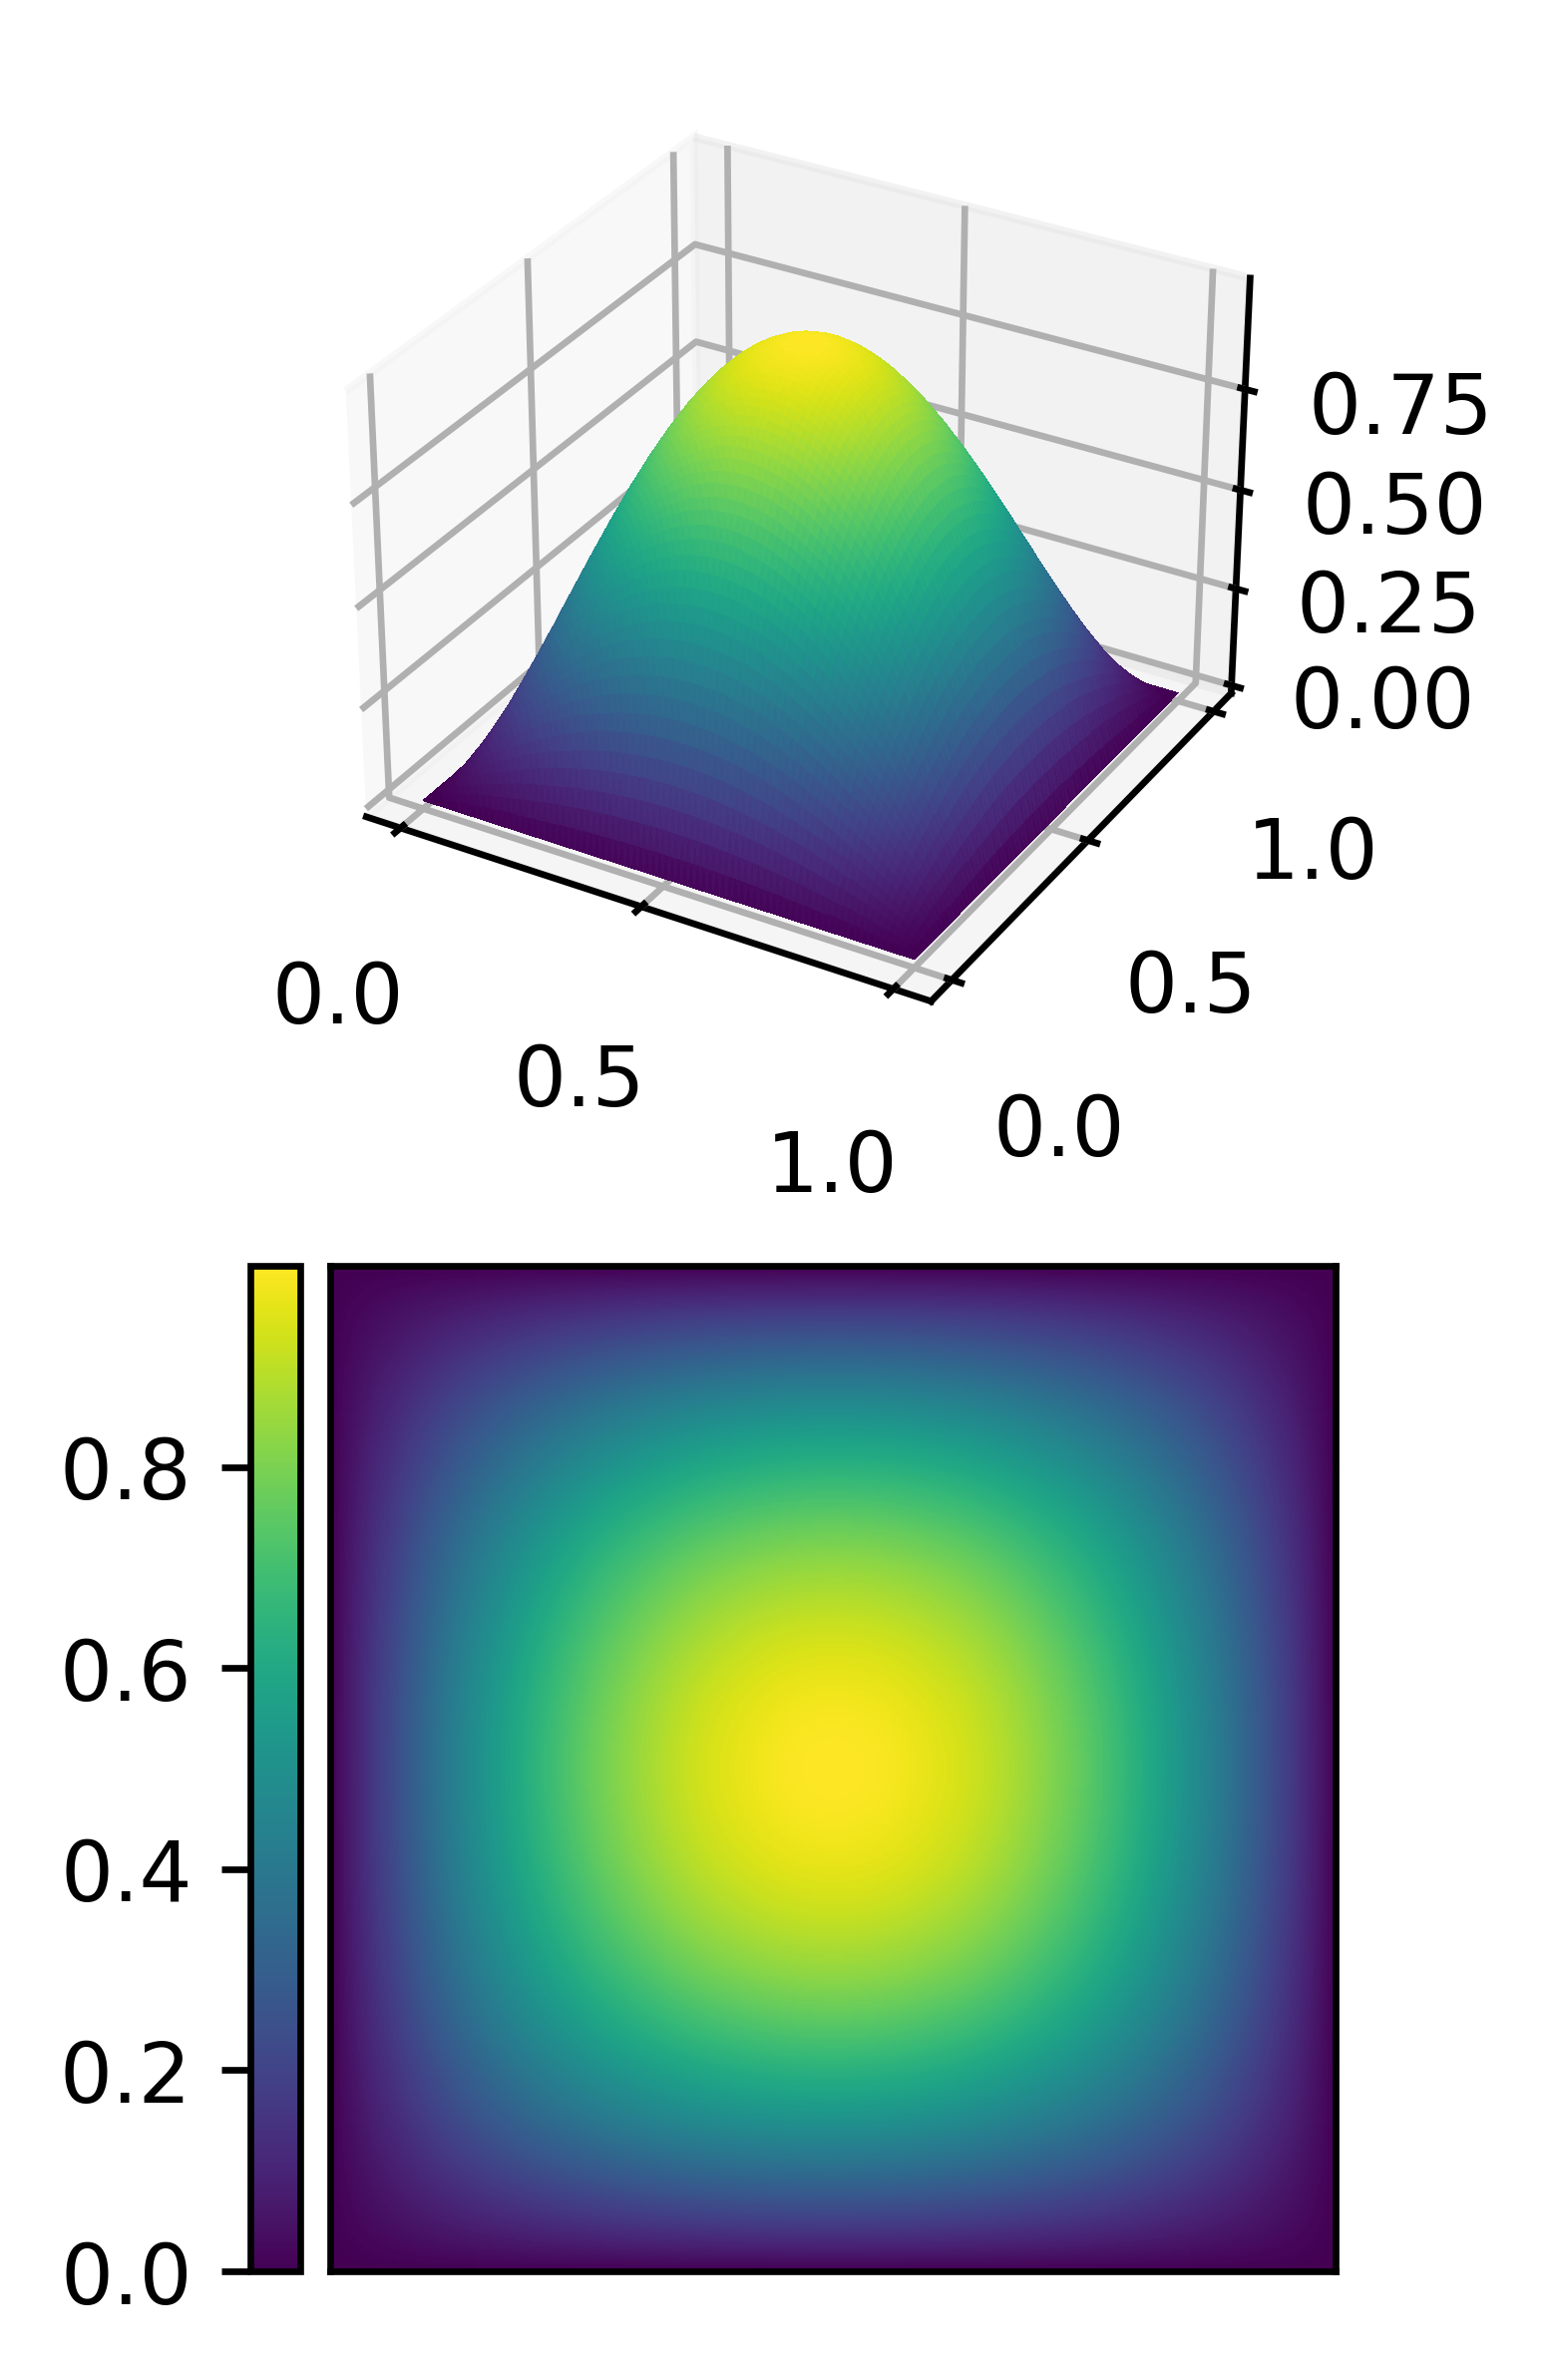
\includegraphics[width=.6\linewidth]{contour_1}
    \caption{$a = 1$}
  \end{subfigure}%
  \begin{subfigure}{.5\textwidth}
    \centering
    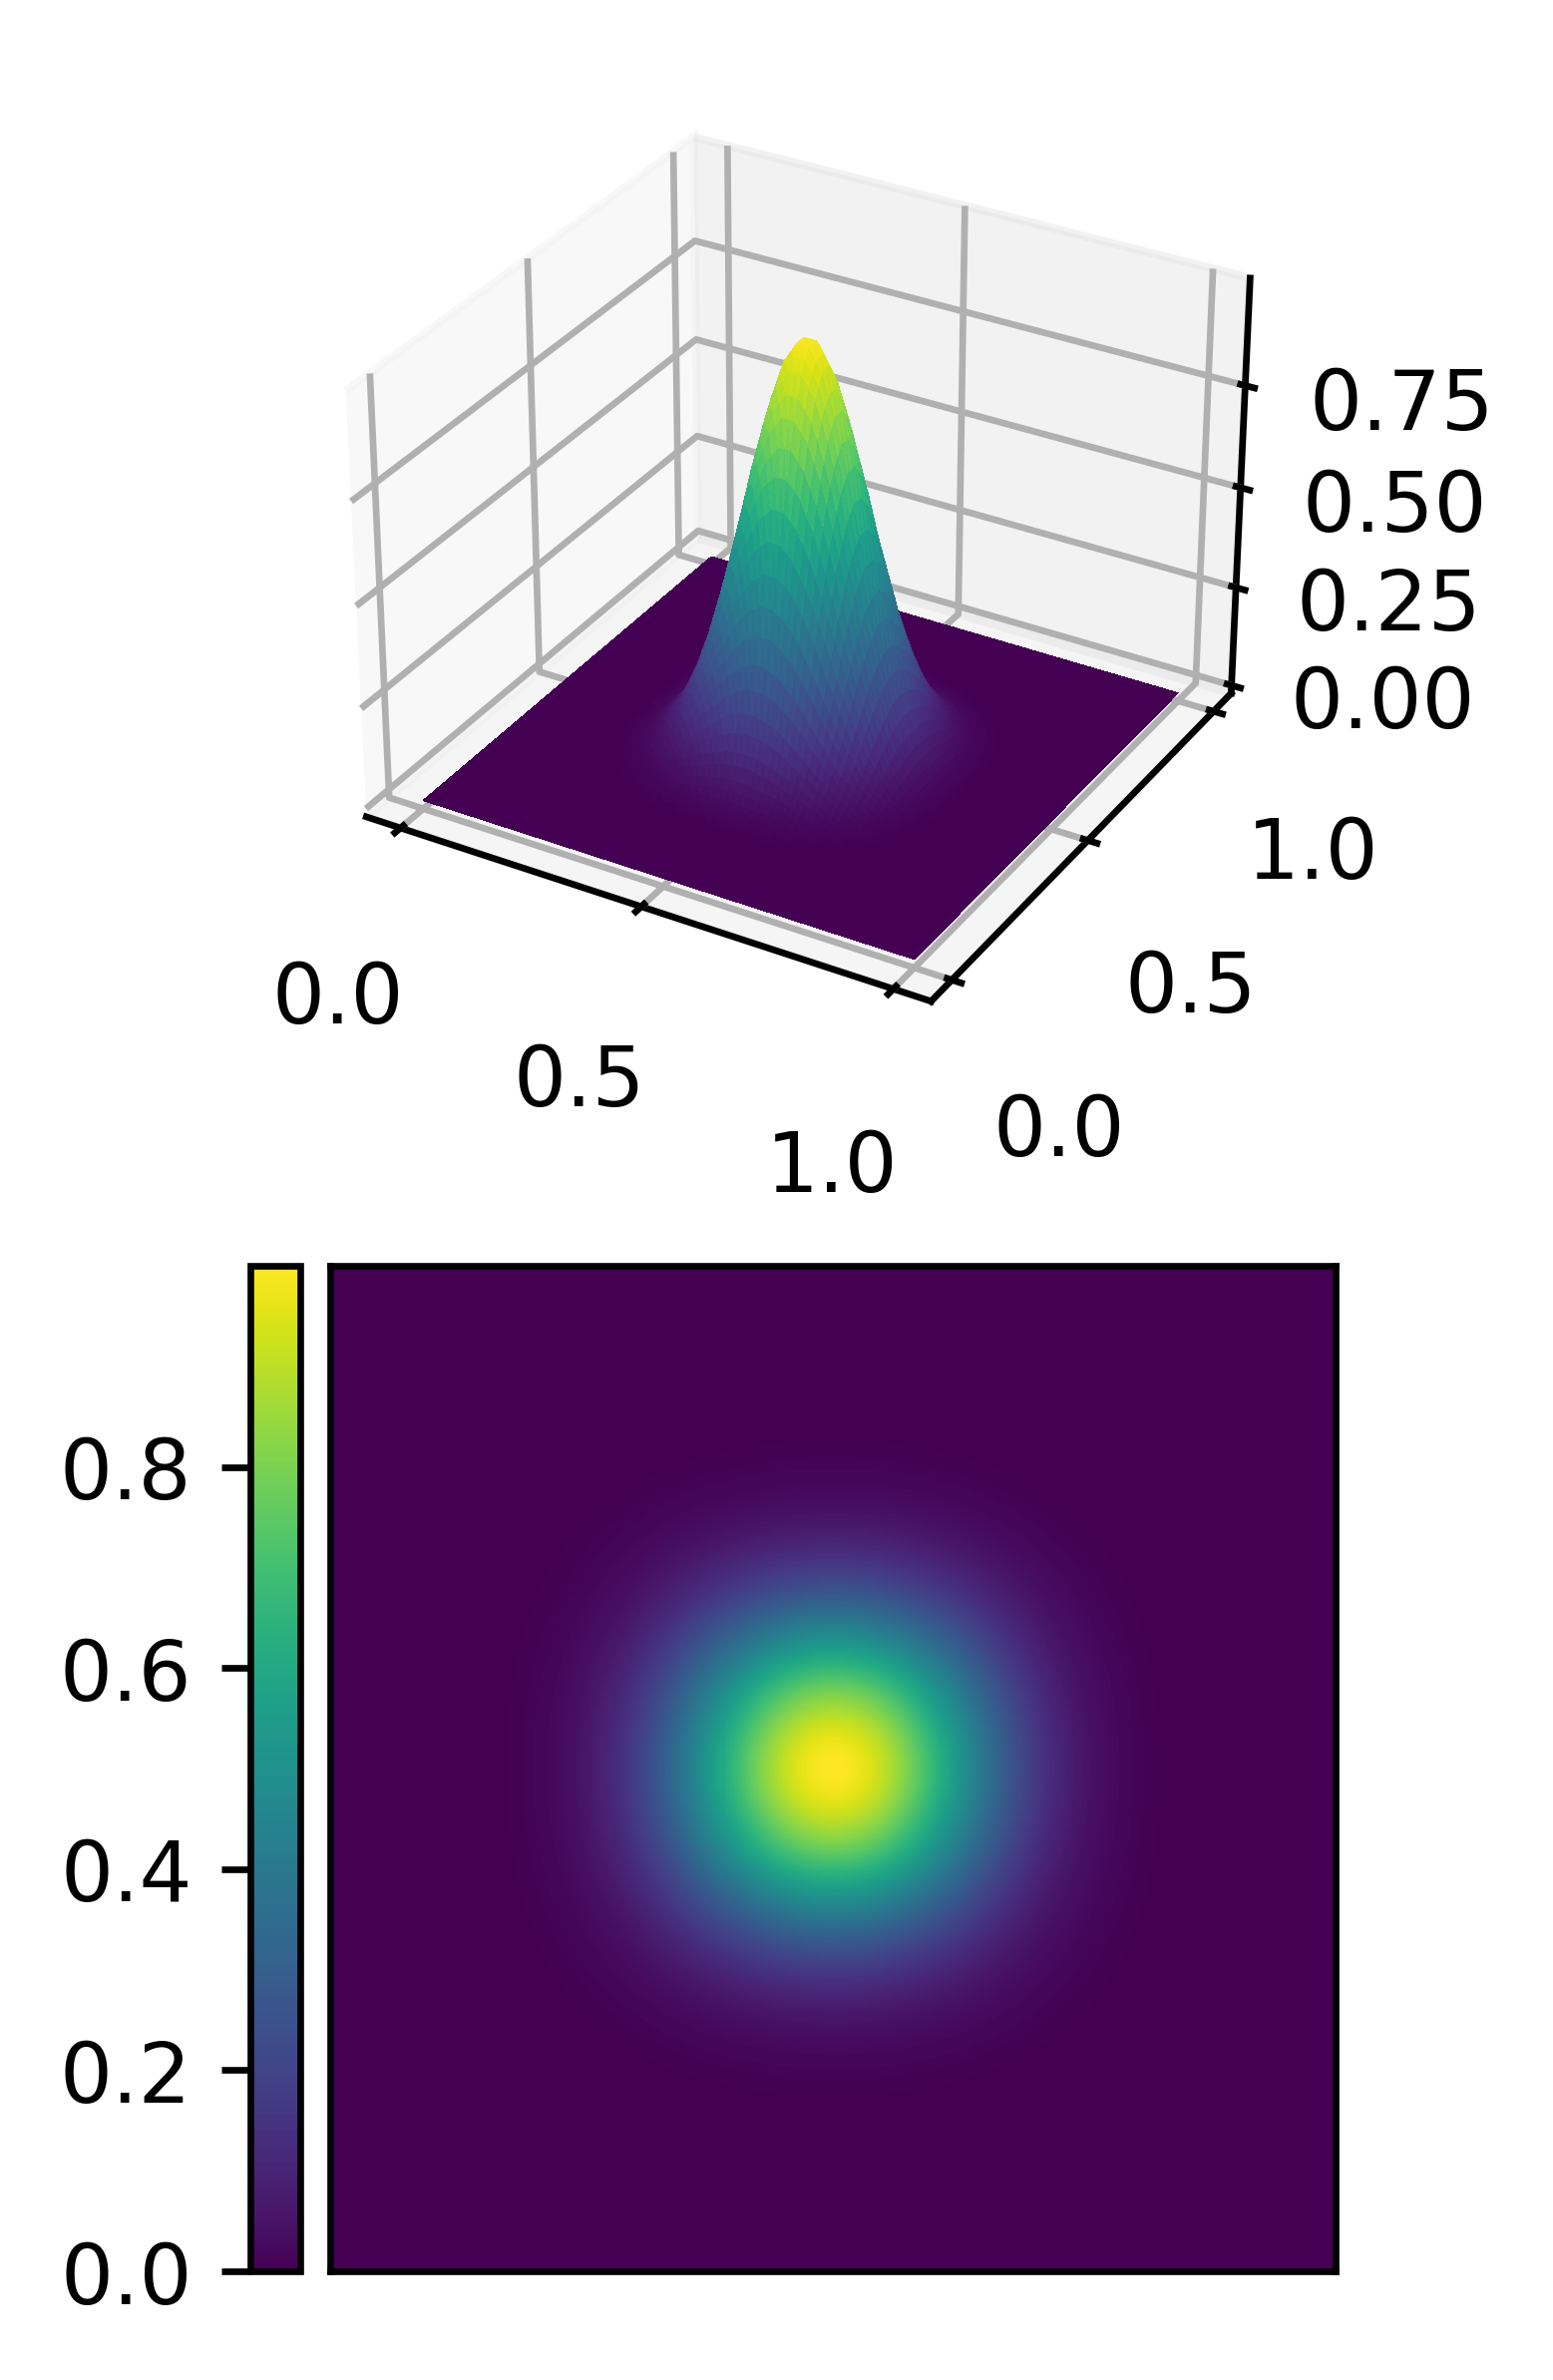
\includegraphics[width=.6\linewidth]{contour_10}
    \caption{$a = 10$}
  \end{subfigure}
  \caption{Solution $u$ with varying parameter $a$}
  \label{fig:smooth_dirichlet_solution}
\end{figure}

\begin{figure}
  \centering
  \begin{subfigure}{.2\textwidth}
    \centering
    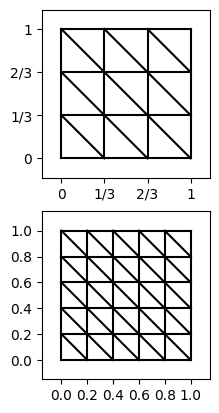
\includegraphics[width=1\linewidth]{structured_grids}
    \caption{Grids for $n=4$ and $n=6$}
  \end{subfigure}%
  \begin{subfigure}{.8\textwidth}
    \centering
    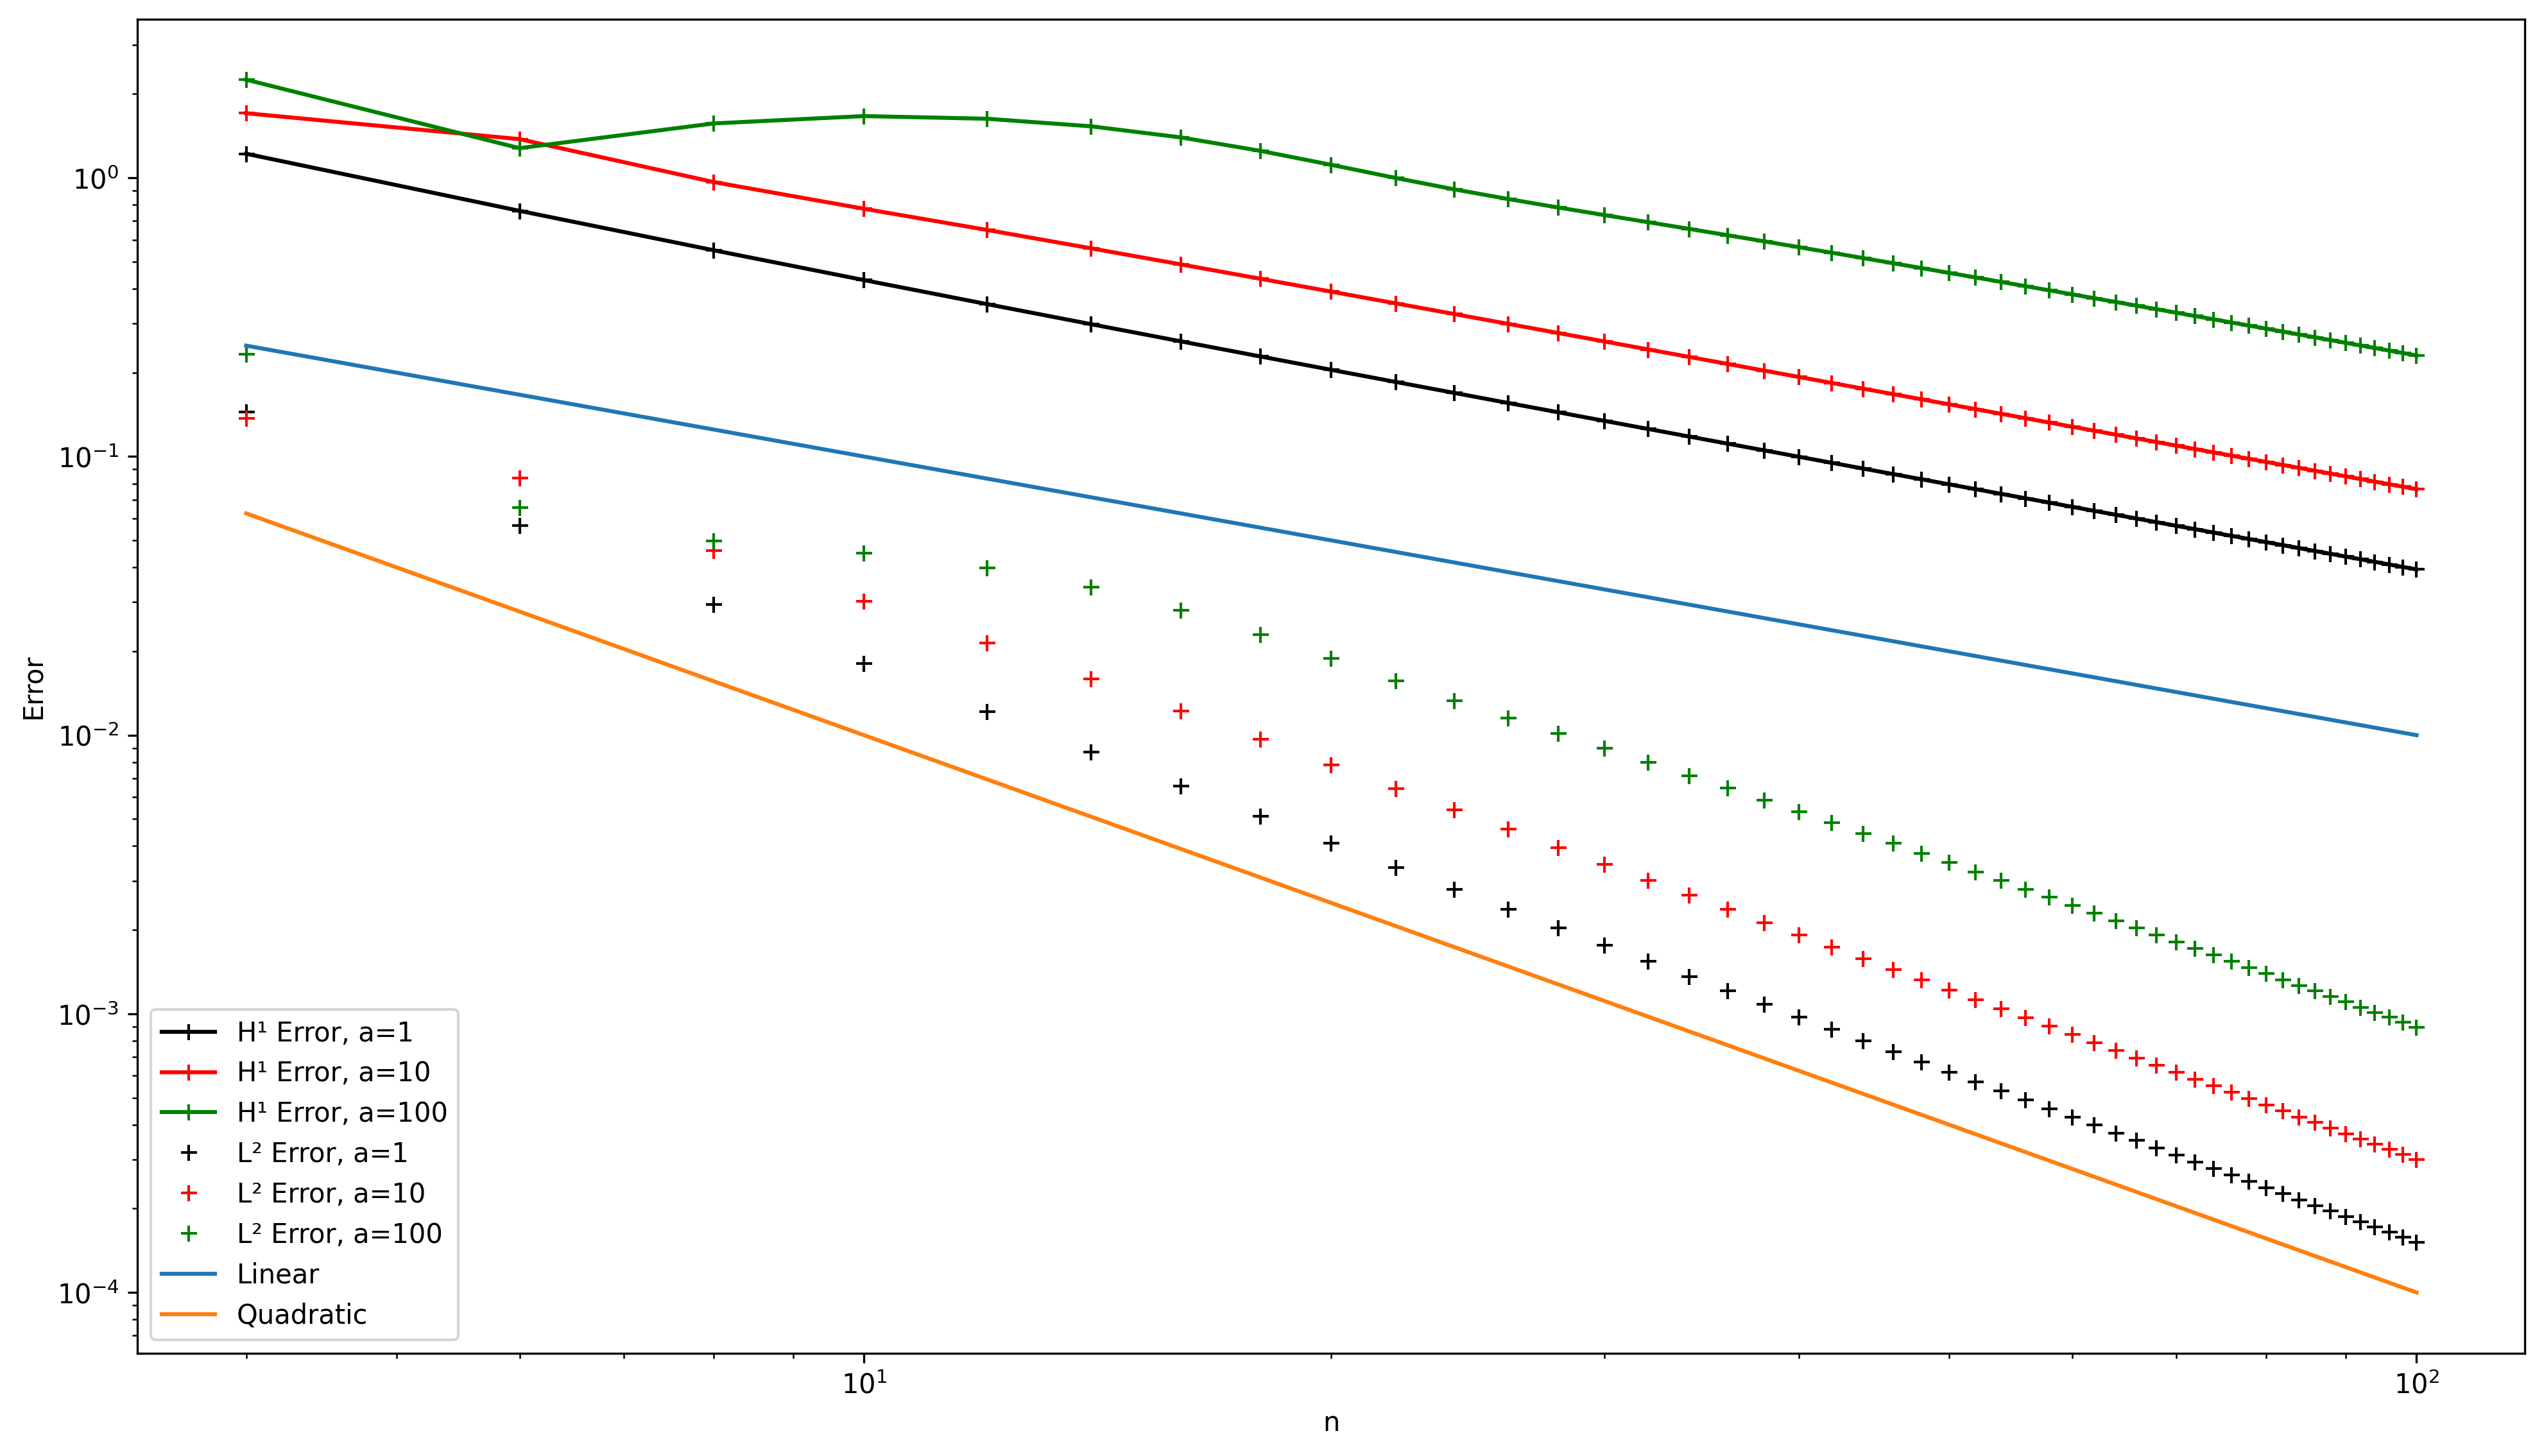
\includegraphics[width=.9\linewidth]{errors_smooth_reg}
    \caption{Error in $L^2$ and $H^1$ Semi-Norm with Gradually Refined Grids and Different $H^2$ Norms of $u$}
  \end{subfigure}
  \label{fig:smooth_dirichlet_str_errs}
  \caption{Smooth Solution with Dirichlet Boundary Conditions on a Structured Grid}
\end{figure}

\begin{figure}
  \centering
  \begin{subfigure}{.2\textwidth}
    \centering
    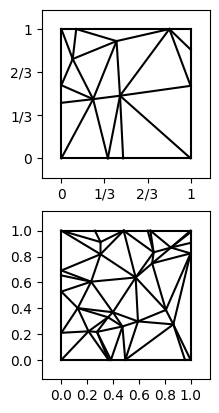
\includegraphics[width=1\linewidth]{unstructured_grids}
    \caption{Grids for $n=4$ and $n=6$}
  \end{subfigure}%
  \begin{subfigure}{.8\textwidth}
    \centering
    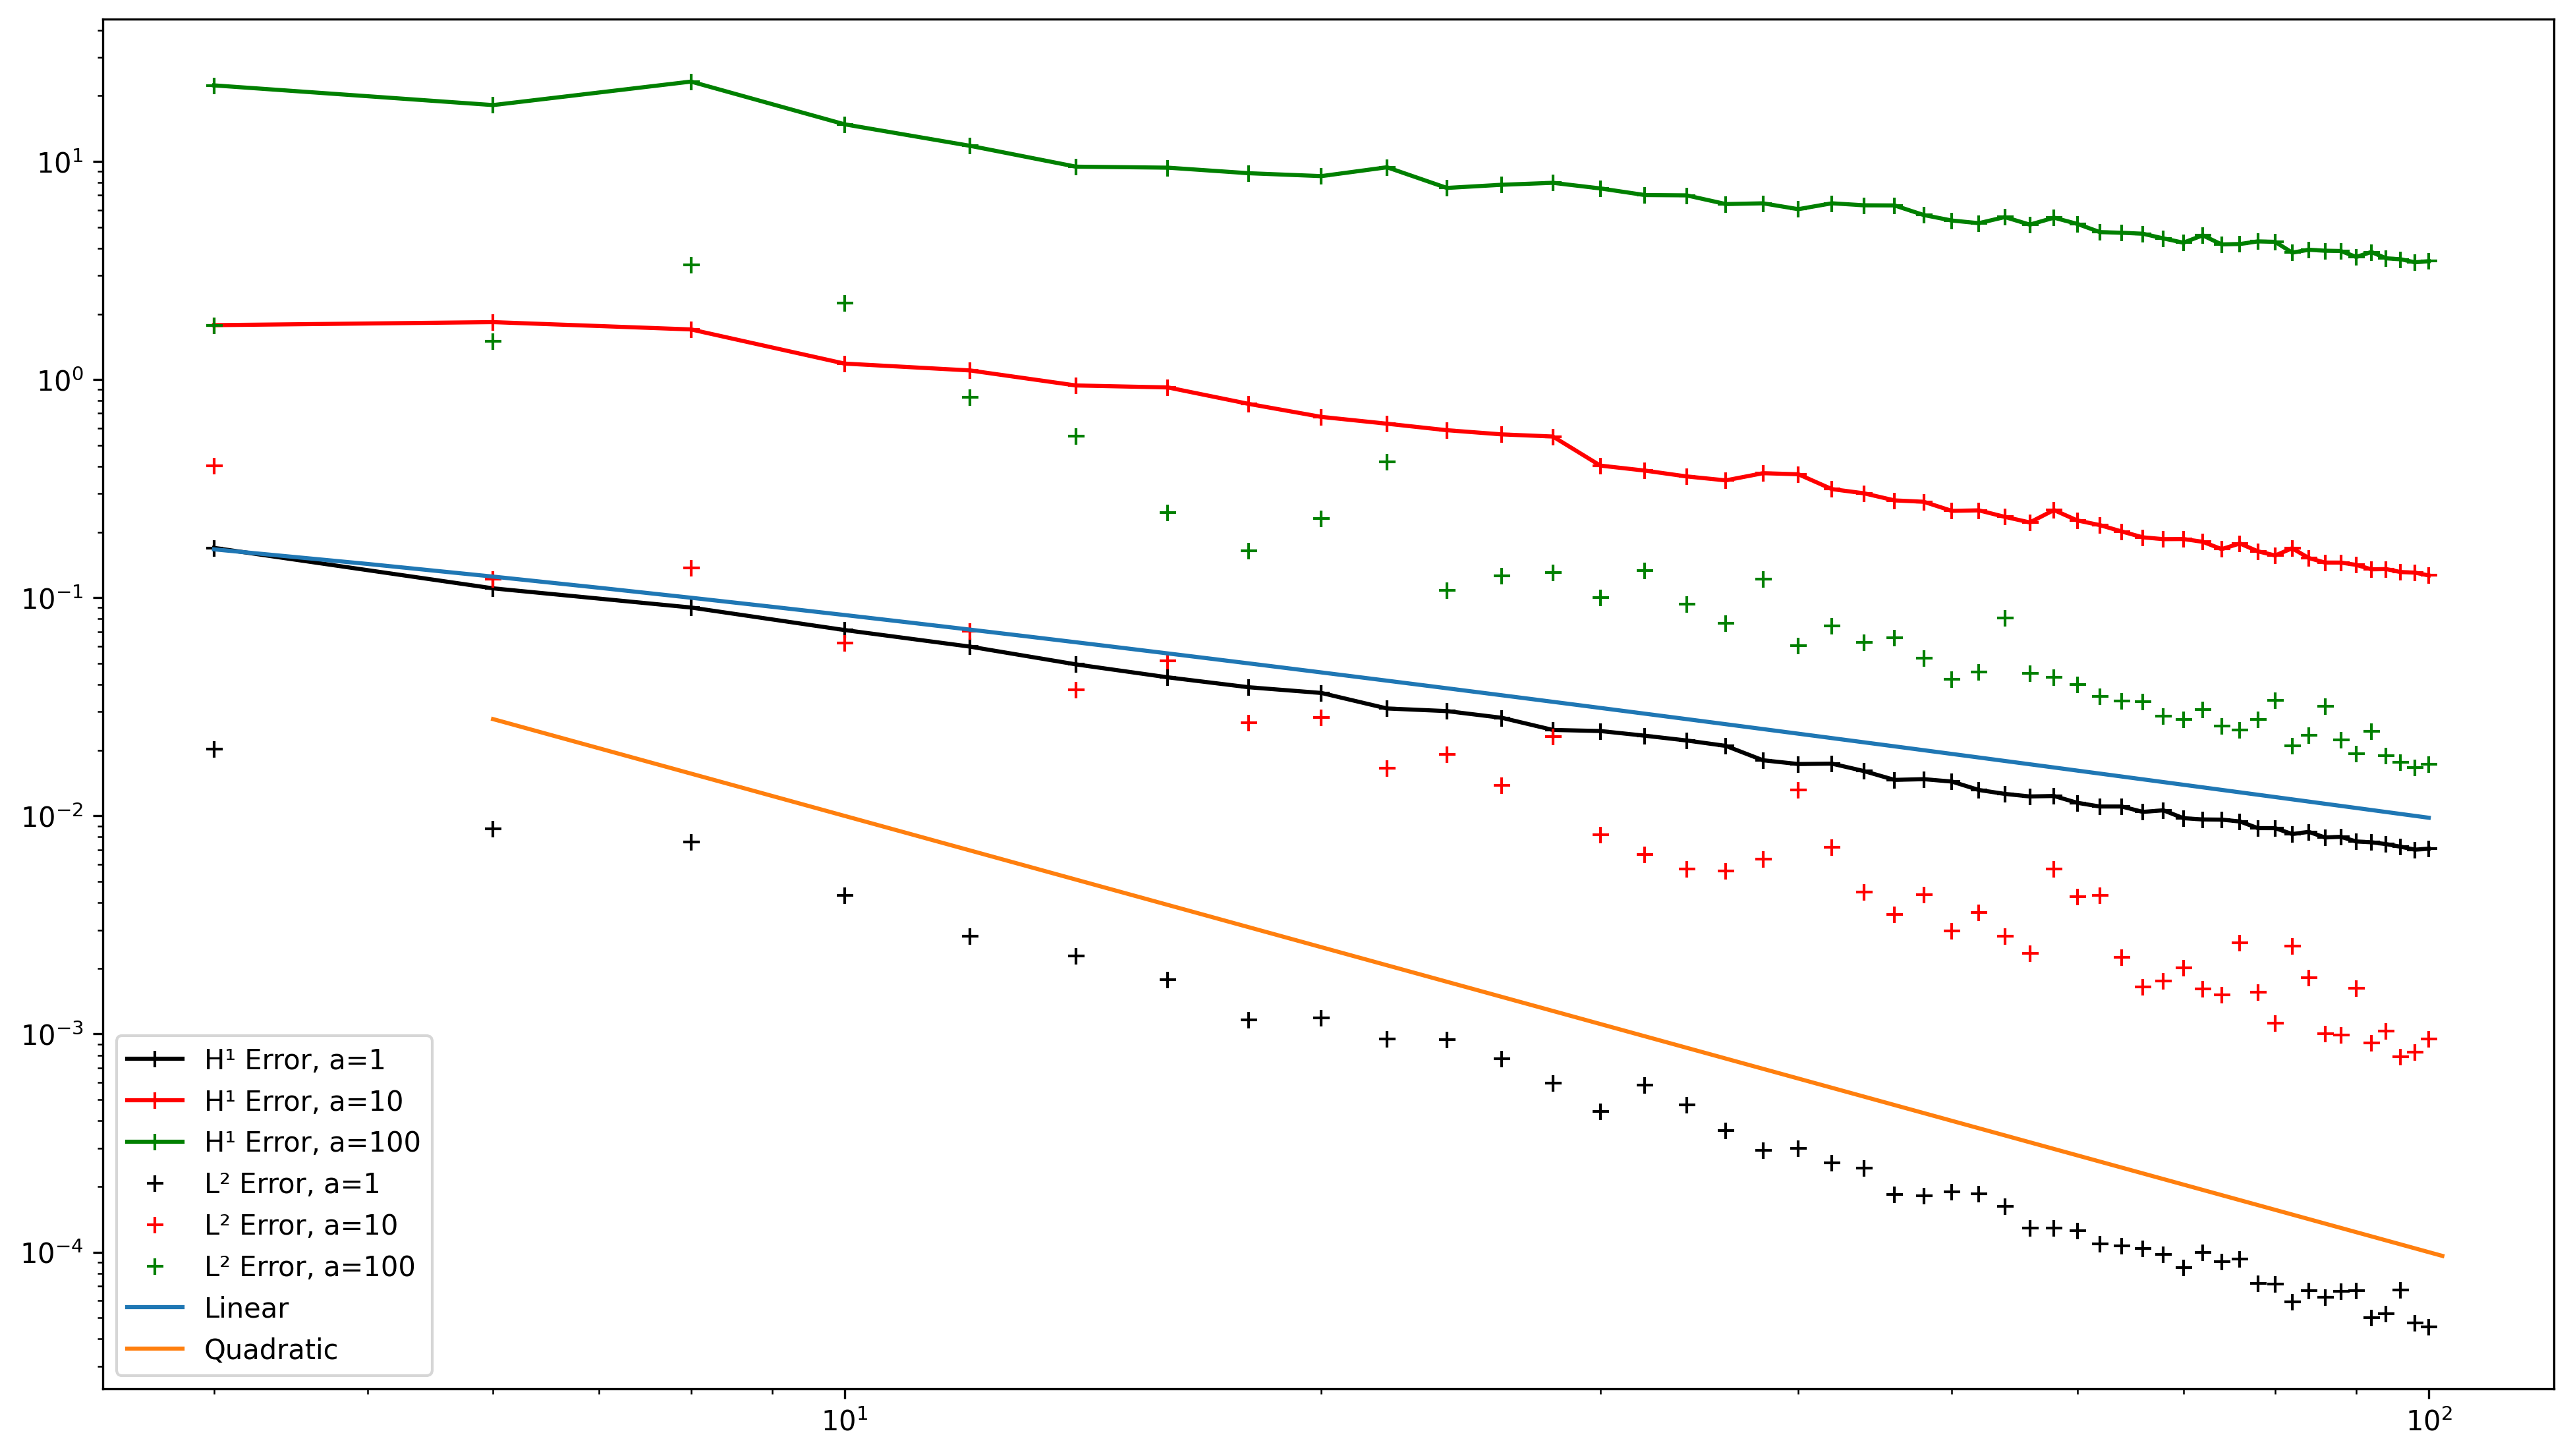
\includegraphics[width=.9\linewidth]{errors_smooth_irreg}
    \caption{Error in $H^1$ Semi-Norm with Increasing $H^2$ Norm of $u$}
  \end{subfigure}
  \label{fig:smooth_dirichlet_unstr_errs}
  \caption{Smooth Solution with Dirichlet Boundary Conditions on an Unstructured Grid}
\end{figure}


\subsection*{Less Regular Forces}
Considering the following problem with mixed Dirichlet and Neumann boundary conditions.
\begin{equation}
  \label{eq:poisson_less_smooth_prob}
  \begin{split}
    \Omega &= \left[-1,1\right]^2\\
    -\Delta u &= \begin{cases}
      \frac{\pi^2}{4} \operatorname{cos}\left(\frac{\pi}{2} \cdot y\right) \quad &x \le 0\\
      \frac{\pi^2}{4} \operatorname{cos}\left(\frac{\pi}{2} \cdot y\right) - a\left(a-1\right)x^{a-2} \quad &x > 0
    \end{cases}\\
    u(x,y) &= 0 \quad \text{on } [-1,0] \times -1 \cup [-1,0] \times 1\\
    u(x,y) &= x^a \quad \text{on } (0,1] \times -1 \cup (0,1] \times 1\\
    \frac{\partial u}{\partial {\bf n}} &= 0 \quad \text{on } -1 \times (-1,1)\\
    \frac{\partial u}{\partial {\bf n}} &= a \quad \text{on } 1 \times (-1,1)
  \end{split}
\end{equation}
With known solution:
\begin{equation*}
  u(x,y) = \begin{cases}
    \operatorname{cos}\left(\frac{\pi}{2} \cdot y\right) \quad &x \le 0\\
    \operatorname{cos}\left(\frac{\pi}{2} \cdot y\right) + x^a \quad &x > 0
  \end{cases}
\end{equation*}

Where $u \in H^{a+0.5 - \epsilon}(\Omega) \quad \forall \epsilon > 0$. With increasing $a$,
the function $\Delta u$ will develop a singularity along the $x = 0$ line. For the previous convergence
results to be meaningful we need $a > 1$, so $u$ is continuous and the interpolation operator
well-defined.\\
The varying regularity of the boundary conditions does not pose a problem, since only boundedness
for the Neumann boundary and square integrability for the Dirichlet boundary is needed.

\begin{figure}
  \centering
  \begin{subfigure}{.5\textwidth}
    \centering
    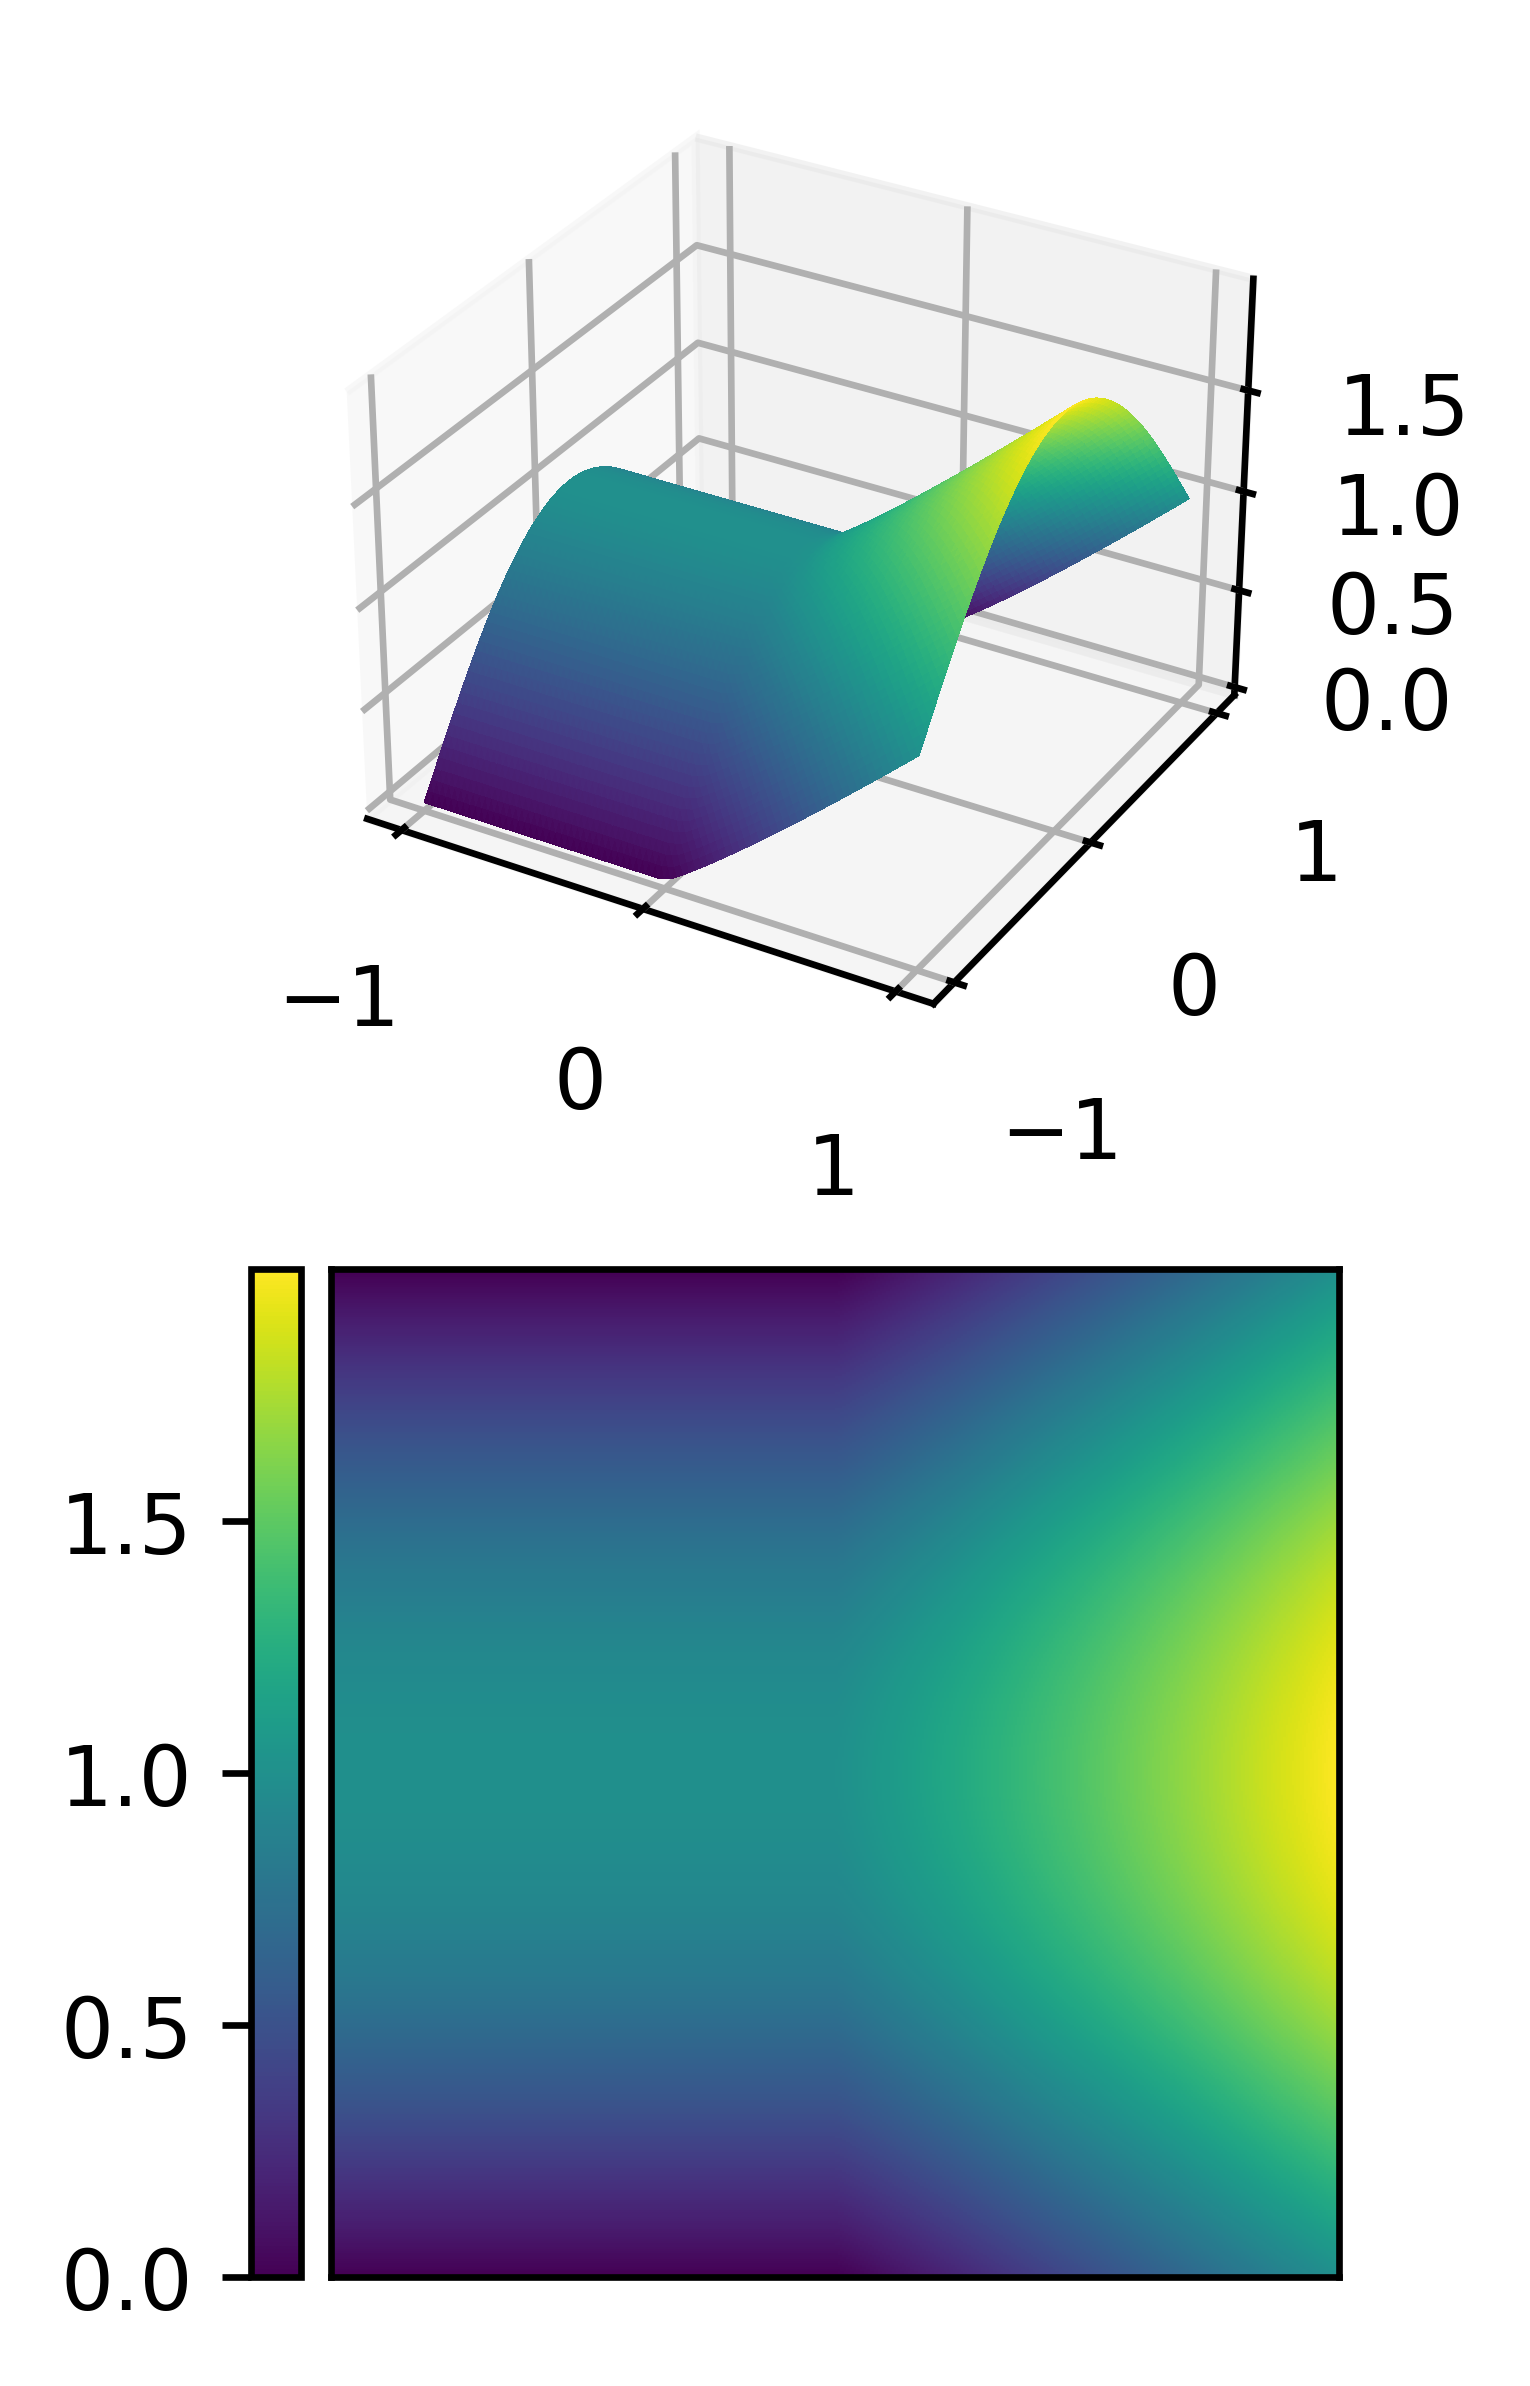
\includegraphics[width=.6\linewidth]{contour_nonsmooth_1}
    \caption{$a = 1.1$}
  \end{subfigure}%
  \begin{subfigure}{.5\textwidth}
    \centering
    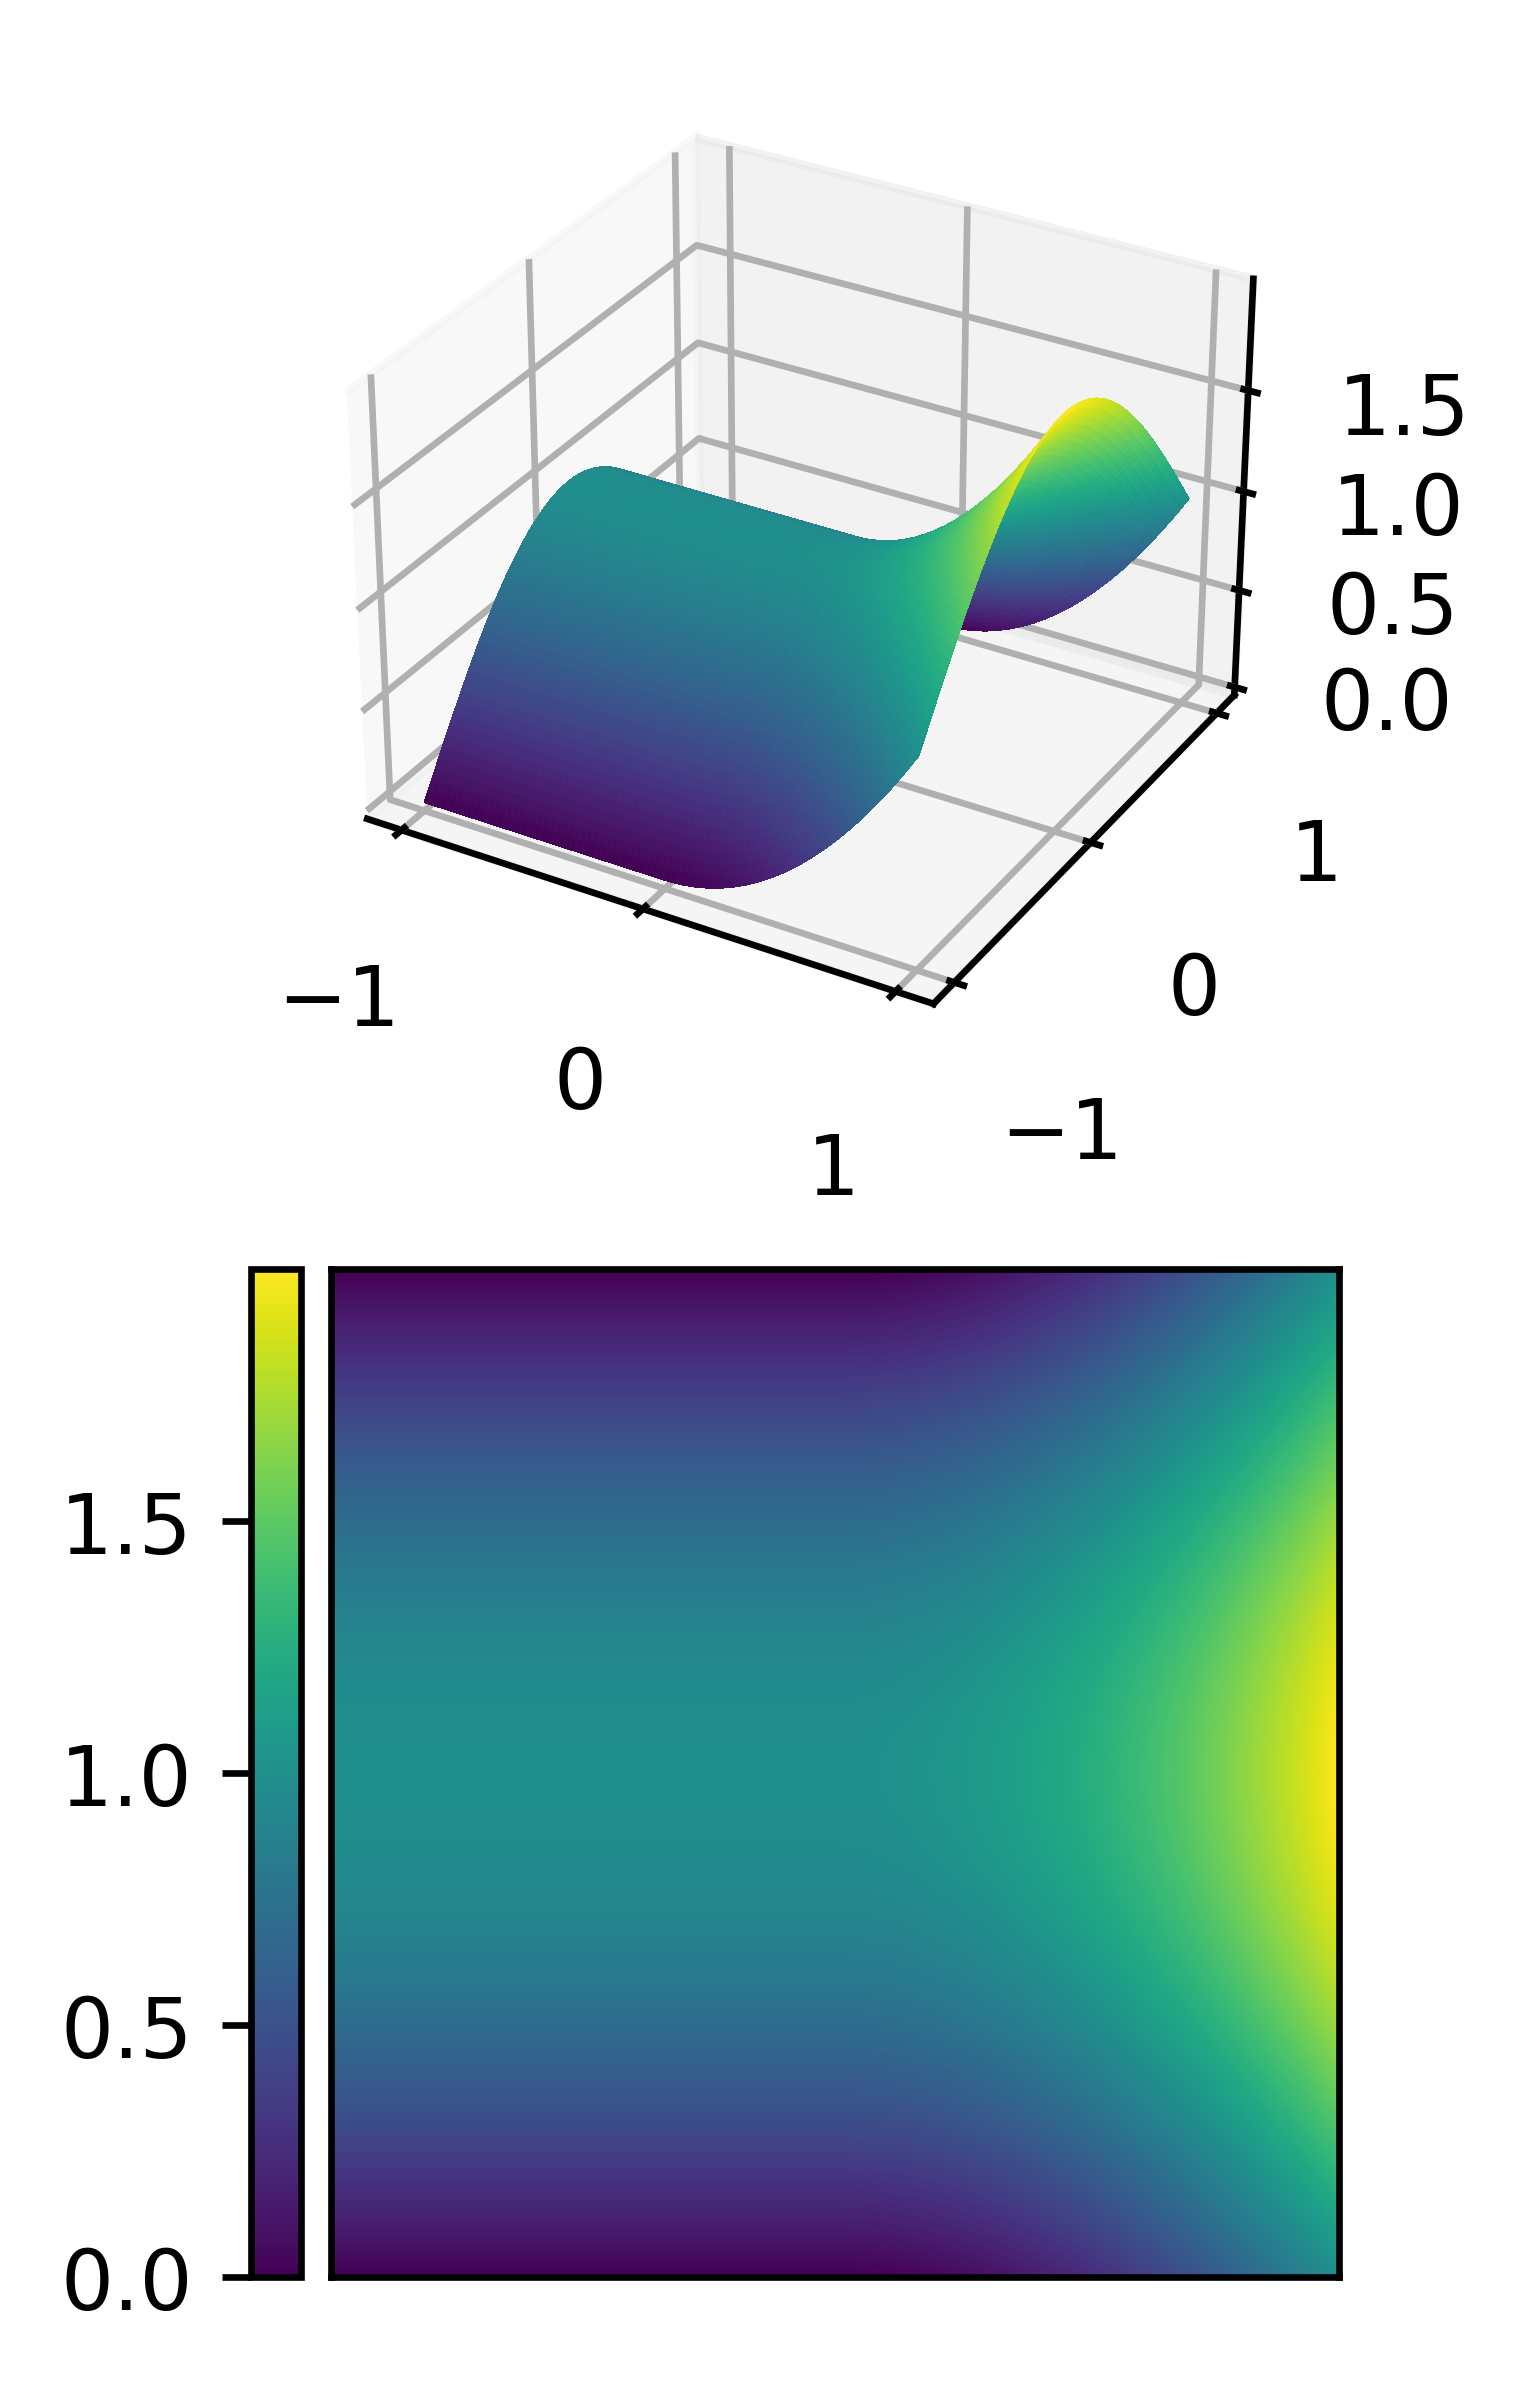
\includegraphics[width=.6\linewidth]{contour_nonsmooth_2}
    \caption{$a = 2$}
  \end{subfigure}
  \caption{Solution $u$ with varying parameter $a$}
  \label{fig:non_smooth_mixed_solution}
\end{figure}

For $1.5 < a$ linear convergence in the $H^1$ semi-norm is expected.
For $1 < a \le 1.5$ we have $u \notin H^2(\Omega)$ and linear convergence in the $L^2$ norm at best.
And for $1.5 < a$ quadratic convergence in the $L^2$ norm at best.
However, the theorem guaranteeing a convergence estimates in its precise form states:
\begin{equation}
  \begin{split}
    &\exists n \in \mathbb{N}: \, \lVert u - u_h \rVert_{L^2} \in \mathcal{O}\left(h\right), \quad \forall h < \frac{1}{n}, u \in H^1(\Omega) \\
    &\exists n \in \mathbb{N}: \, \lVert u - u_h \rVert_{L^2} \in \mathcal{O}\left(h^2\right), \quad \forall h < \frac{1}{n}, u \in H^2(\Omega) \\
  \end{split}
\end{equation}
This threshold is likely to increase with less regularity of the solution. So a more natural
expectation is for the convergence rate to increase with increasing $a$.

Both of this is observed in the numerical experiment. As visualized in \ref{fig:err_nonsmooth_h1},
the convergence rate for the $H^1$ semi-norm is exactly linear for $1.5 < a$.
For $a = 1.3$ the method is still guaranteed to converge in the $H^1$ semi-norm, although no convergence estimate can be established.
From the numerical experiment it appears to converge at a rate $\mathcal{O}\left(h^{0.6}\right)$.

In \ref{fig:err_nonsmooth_l2} it can be seen how the convergence rate depends on the regularity of the solution.
For the highly irregular solution with $a = 1.3$, linear convergence is only given during the first steps.
A similar behaviour is observed for $1.5 < a < 2.2$ where quadratic convergence is expected, but only given
during the first steps.
Truly quadratic convergence can only be observed for $2.2 < a$
\begin{figure}
  \centering
  \begin{subfigure}{1\textwidth}
    \centering
    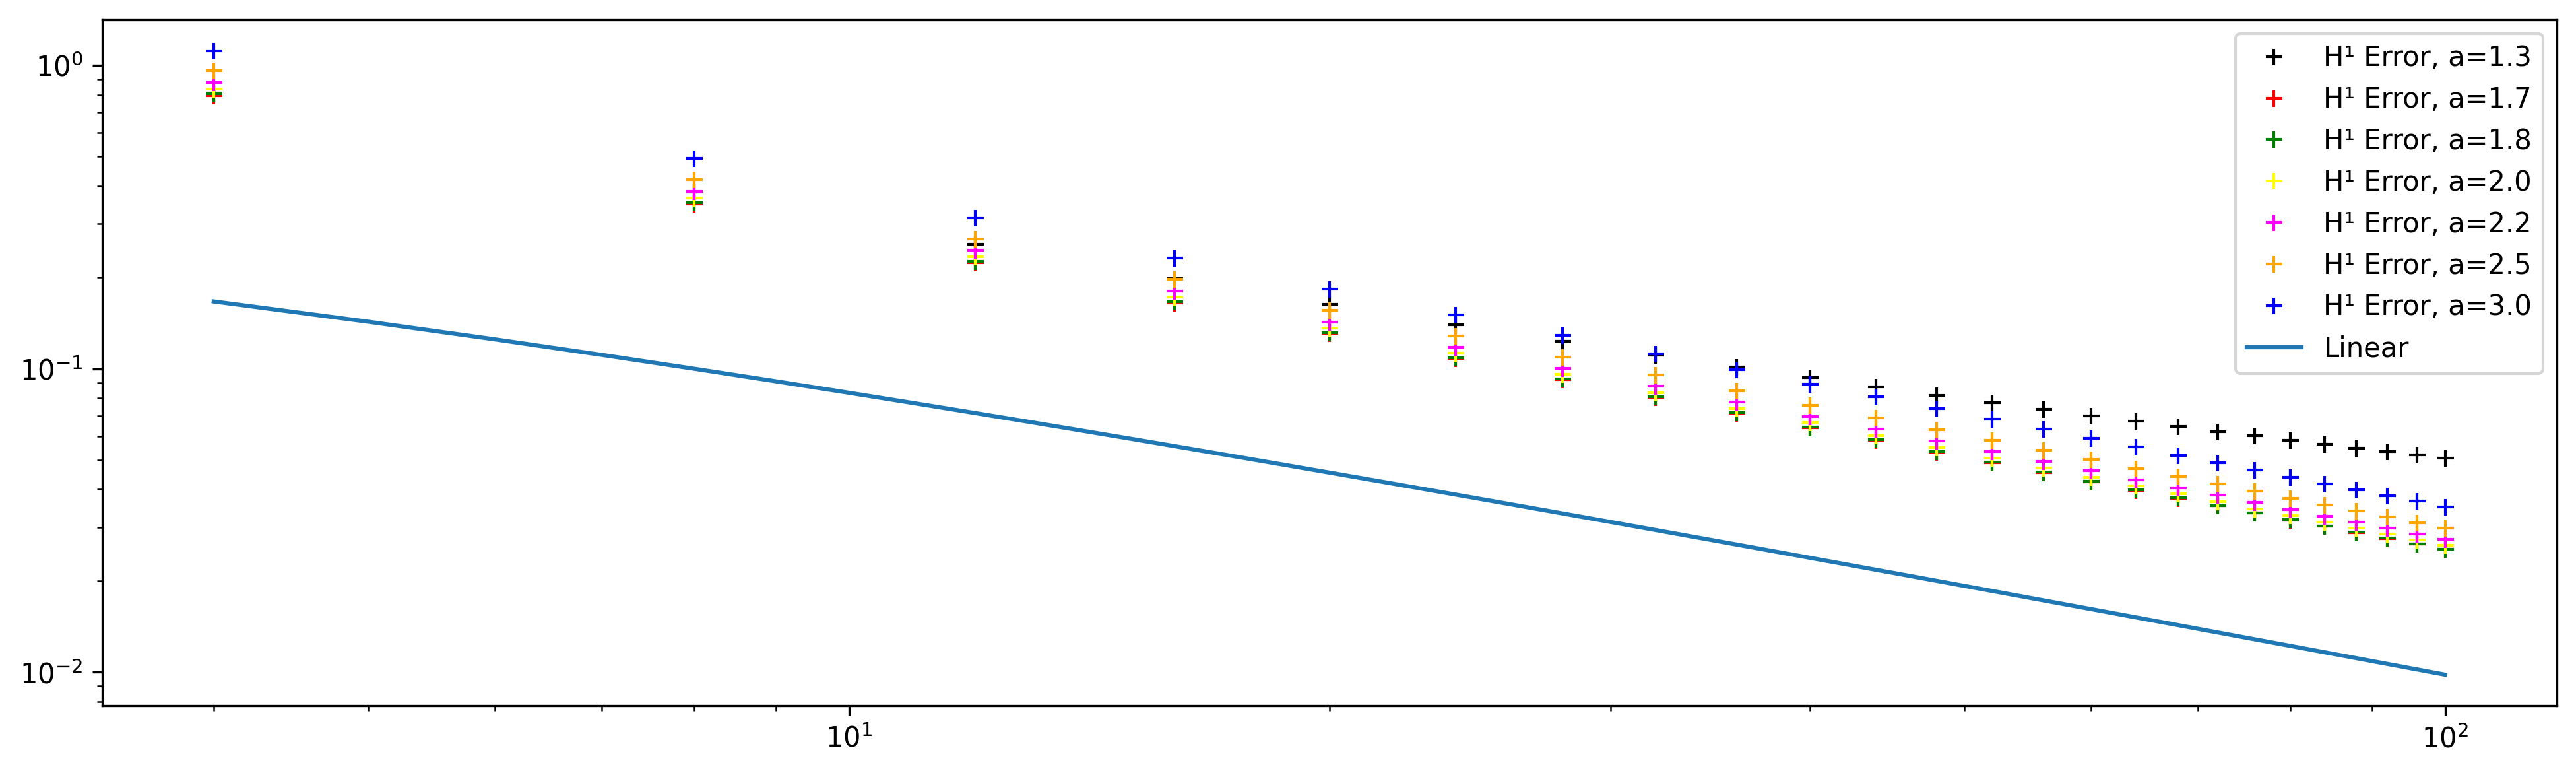
\includegraphics[width=.8\linewidth]{errors_nonsmooth_h1}
    \caption{Convergence in the $H^1$ Semi-Norm}
    \label{fig:err_nonsmooth_h1}
  \end{subfigure}

  \begin{subfigure}{1\textwidth}
    \centering
    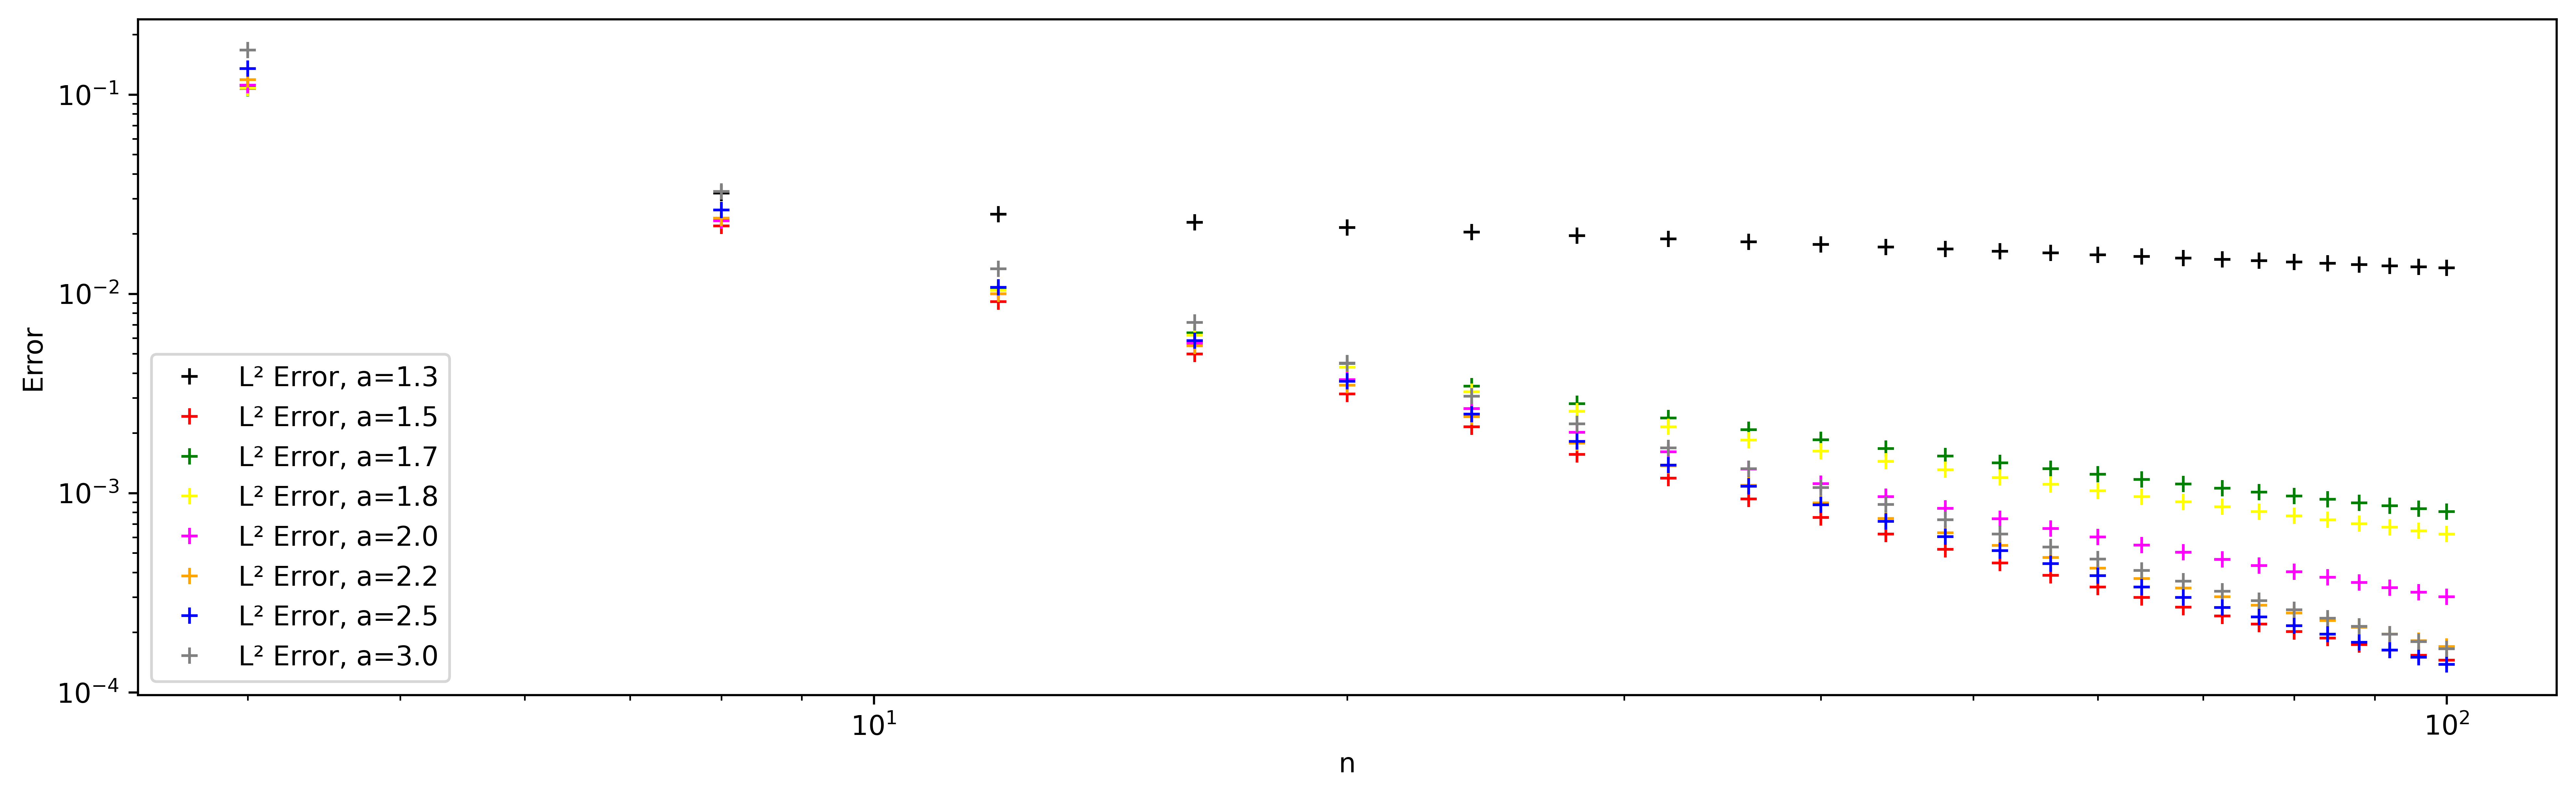
\includegraphics[width=.8\linewidth]{errors_nonsmooth_l2}
    \caption{Convergence in the $L^2$ Norm}
    \label{fig:err_nonsmooth_l2}
  \end{subfigure}
  \caption{Convergence With Varying Regularity of the Solution}
\end{figure}


\subsection*{Higher Order Elements}
To increase the accuracy of the solution on a coarser mesh, a polynomial basis
of higher order can be chosen. This can be achieved by considering higher order local
basis functions defined on the reference element. The local basis functions on the reference
element in 1 and 2 dimension are visualized for 1, 2 and 3 order polynomials in \ref{fig:basis_1d}
and \ref{fig:basis_2d}.

Higher order polynomial basis functions are omitted as the number of basis functions increases quite fast.

\begin{figure}
  \centering
  \begin{subfigure}{1.\textwidth}
    \centering
    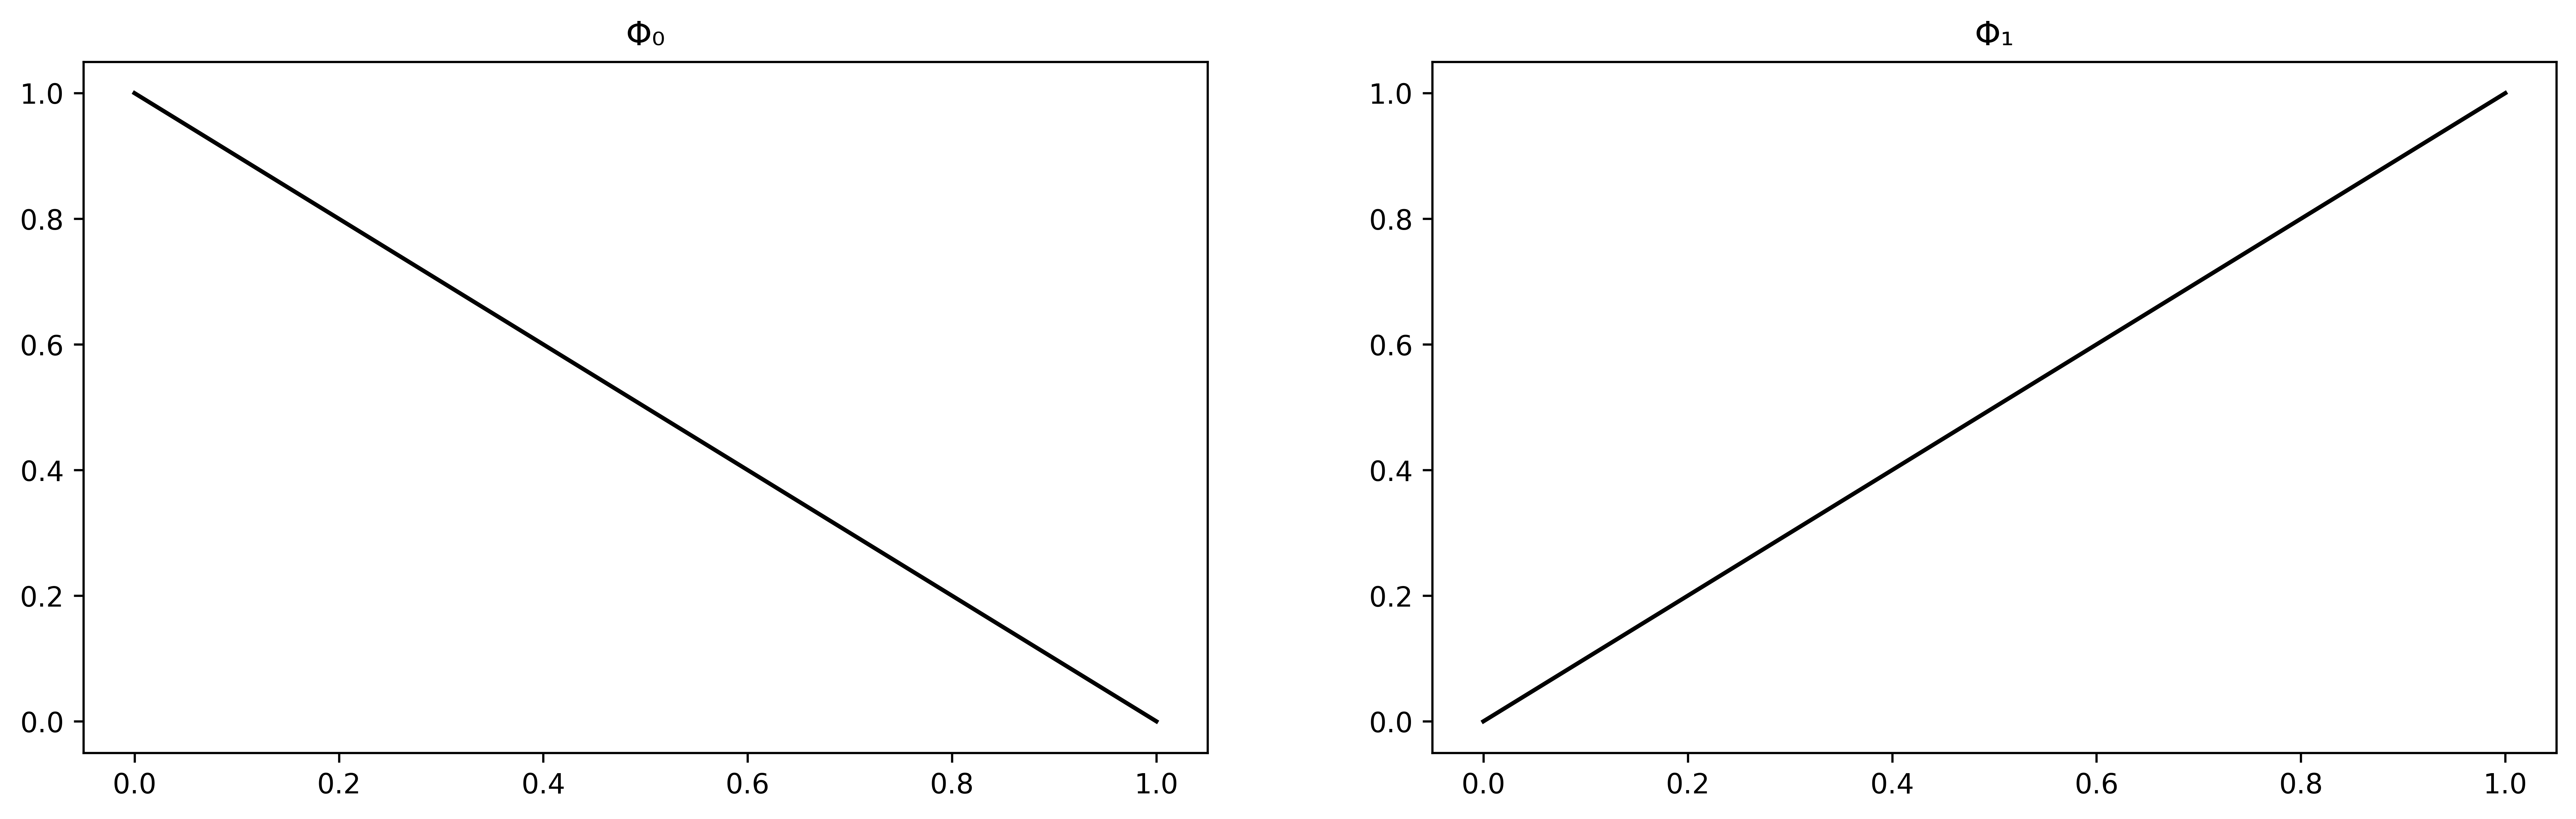
\includegraphics[width=.8\linewidth]{p1_mesh_basis}
    \caption{Polynomial of degree 1 on the unit interval}
  \end{subfigure}
  \begin{subfigure}{1.\textwidth}
    \centering
    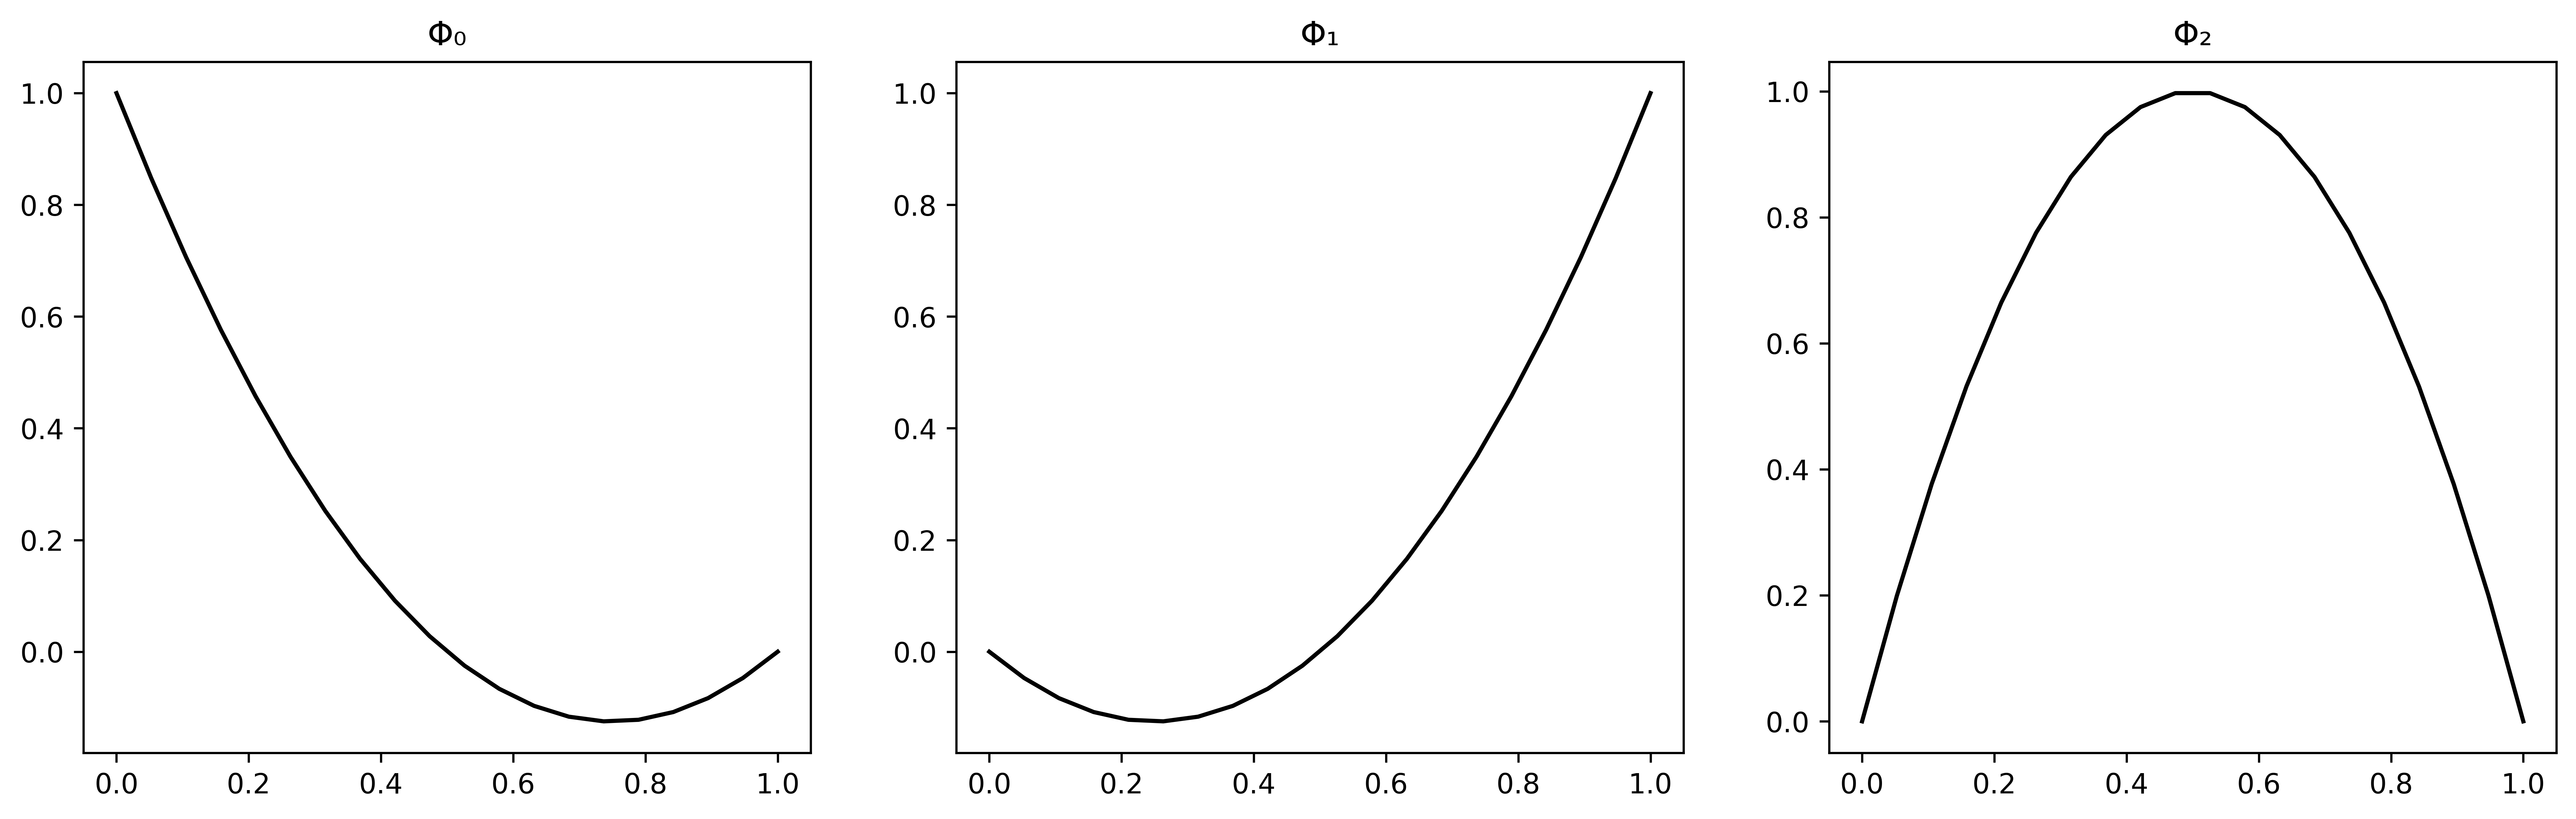
\includegraphics[width=.8\linewidth]{p2_mesh_basis}
    \caption{Polynomial of degree 2 on the unit interval}
  \end{subfigure}
  \begin{subfigure}{1.\textwidth}
    \centering
    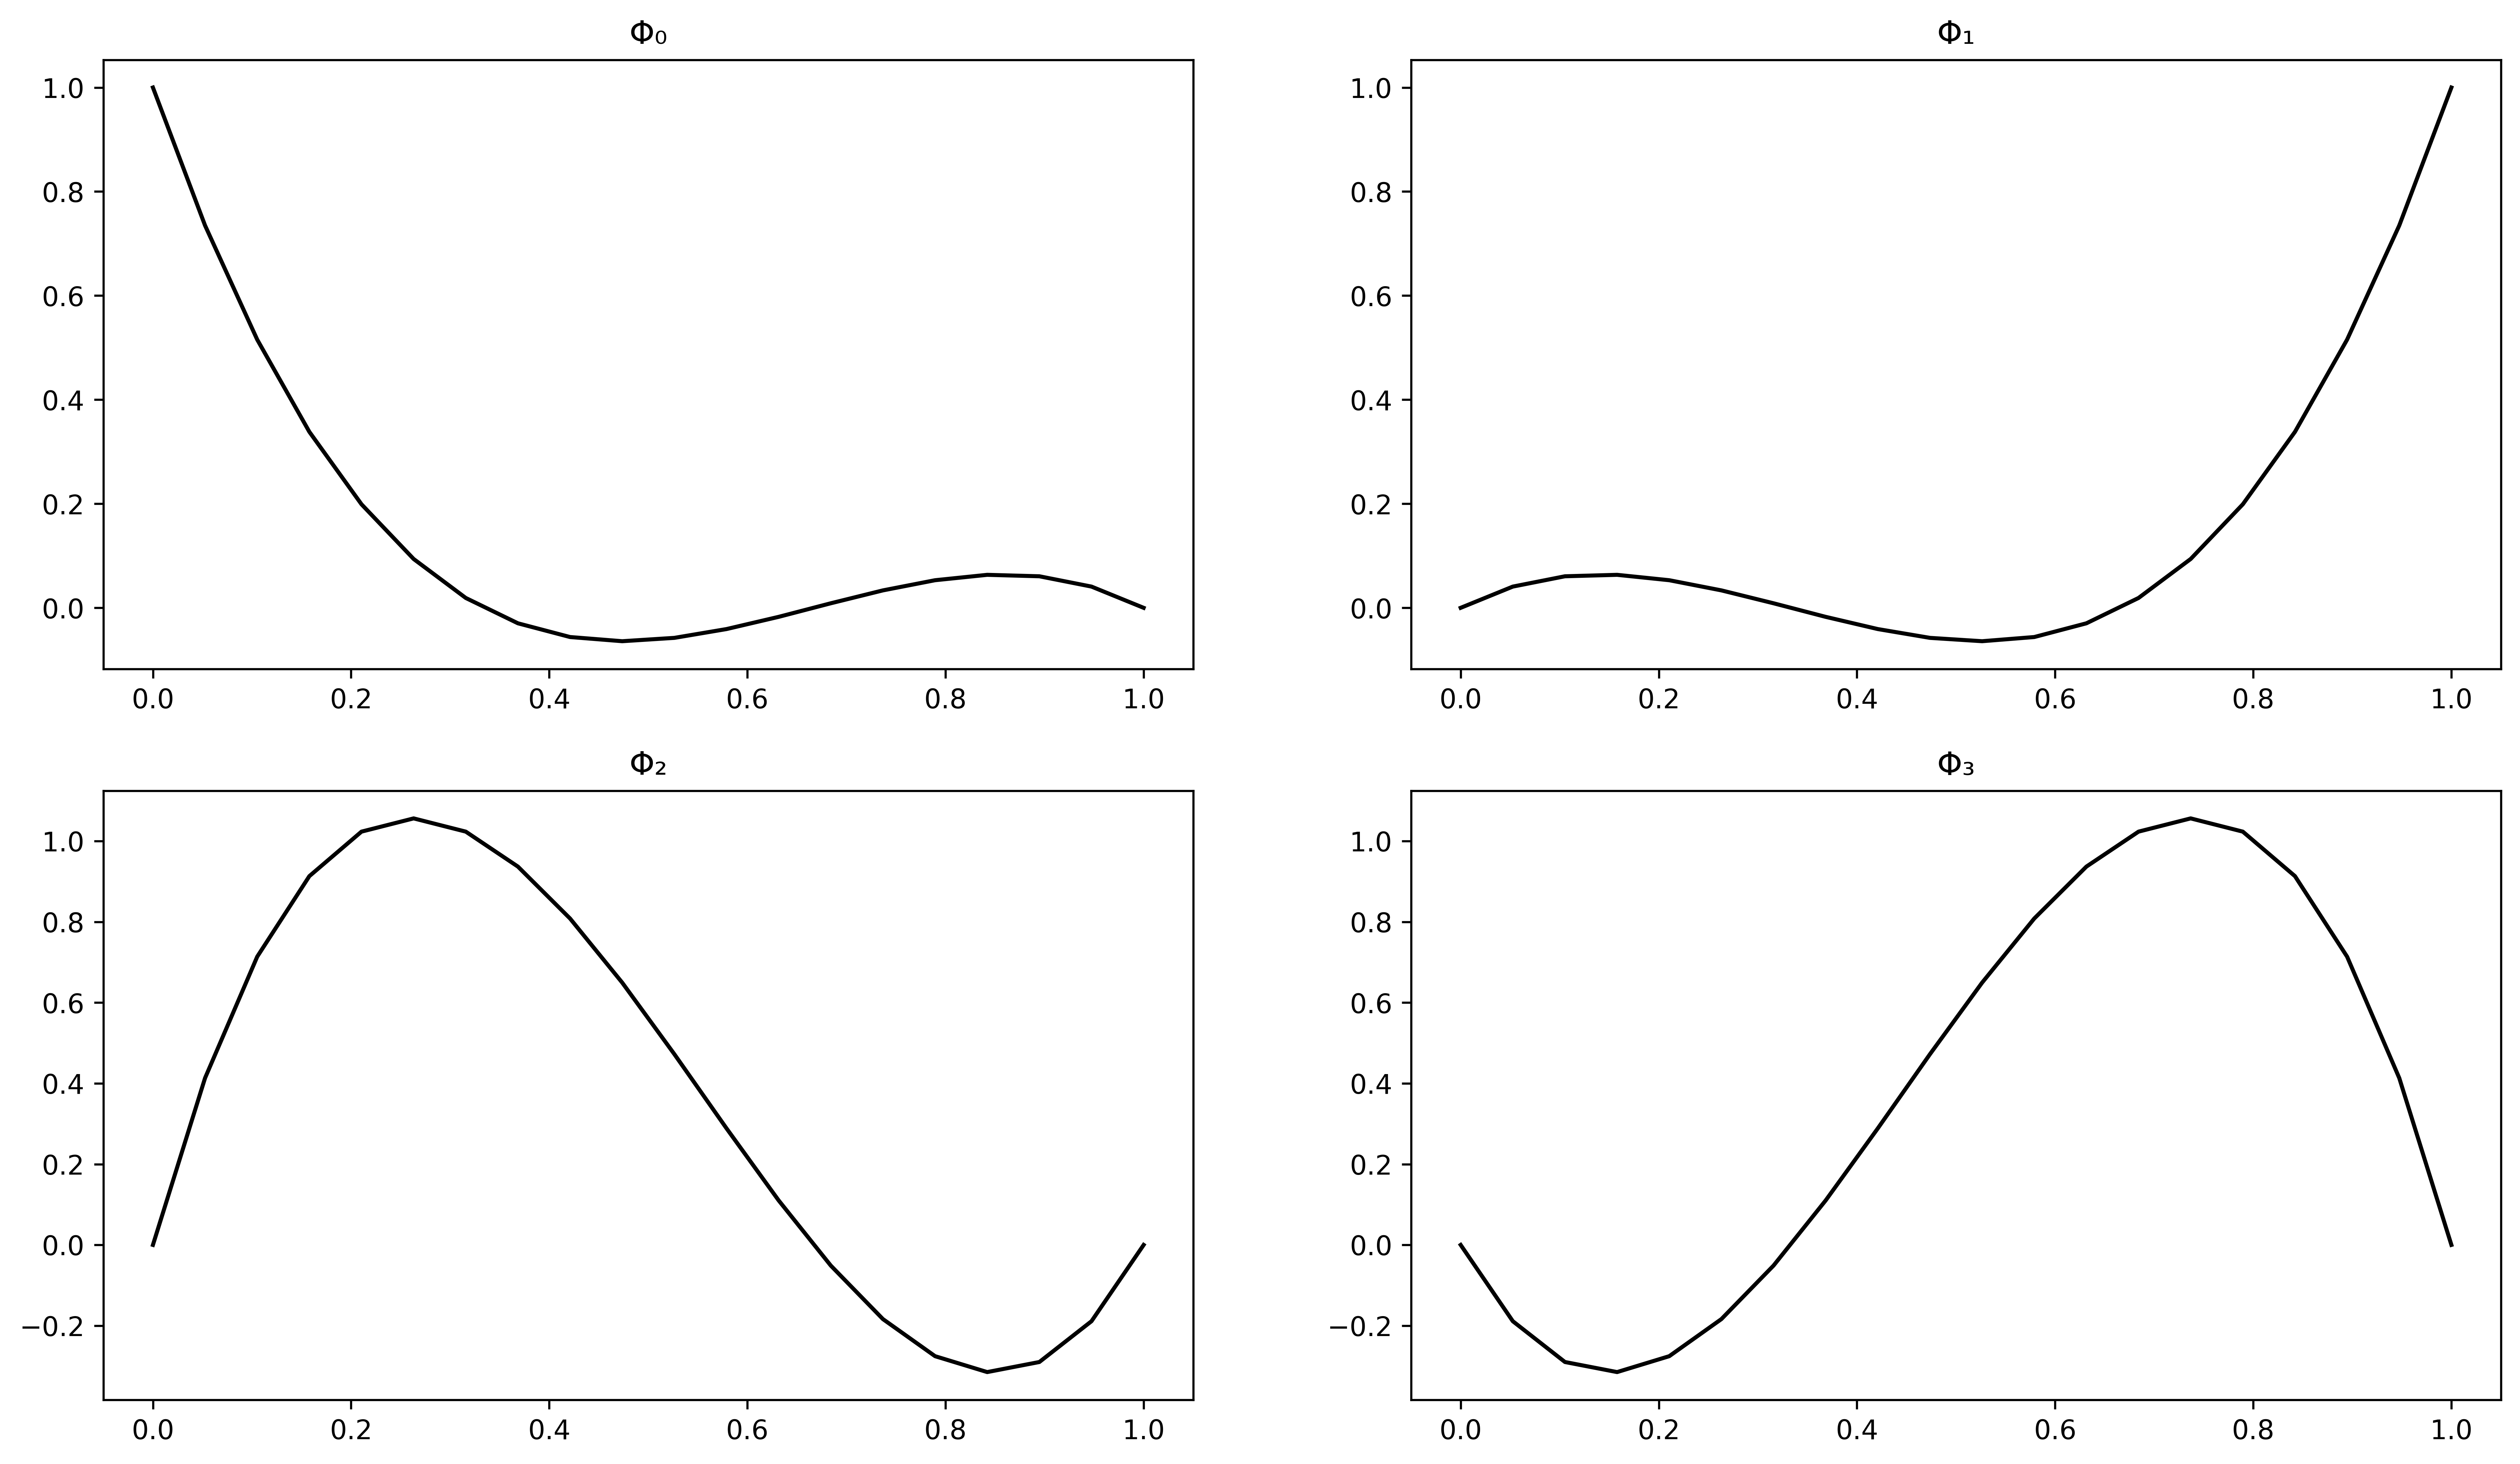
\includegraphics[width=.8\linewidth]{p3_mesh_basis}
    \caption{Polynomial of degree 3 on the unit interval}
  \end{subfigure}
  \caption{Polynomial basis on the 1d reference element}
  \label{fig:basis_1d}
\end{figure}


\begin{figure}
  \centering
  \begin{subfigure}{1.\textwidth}
    \centering
    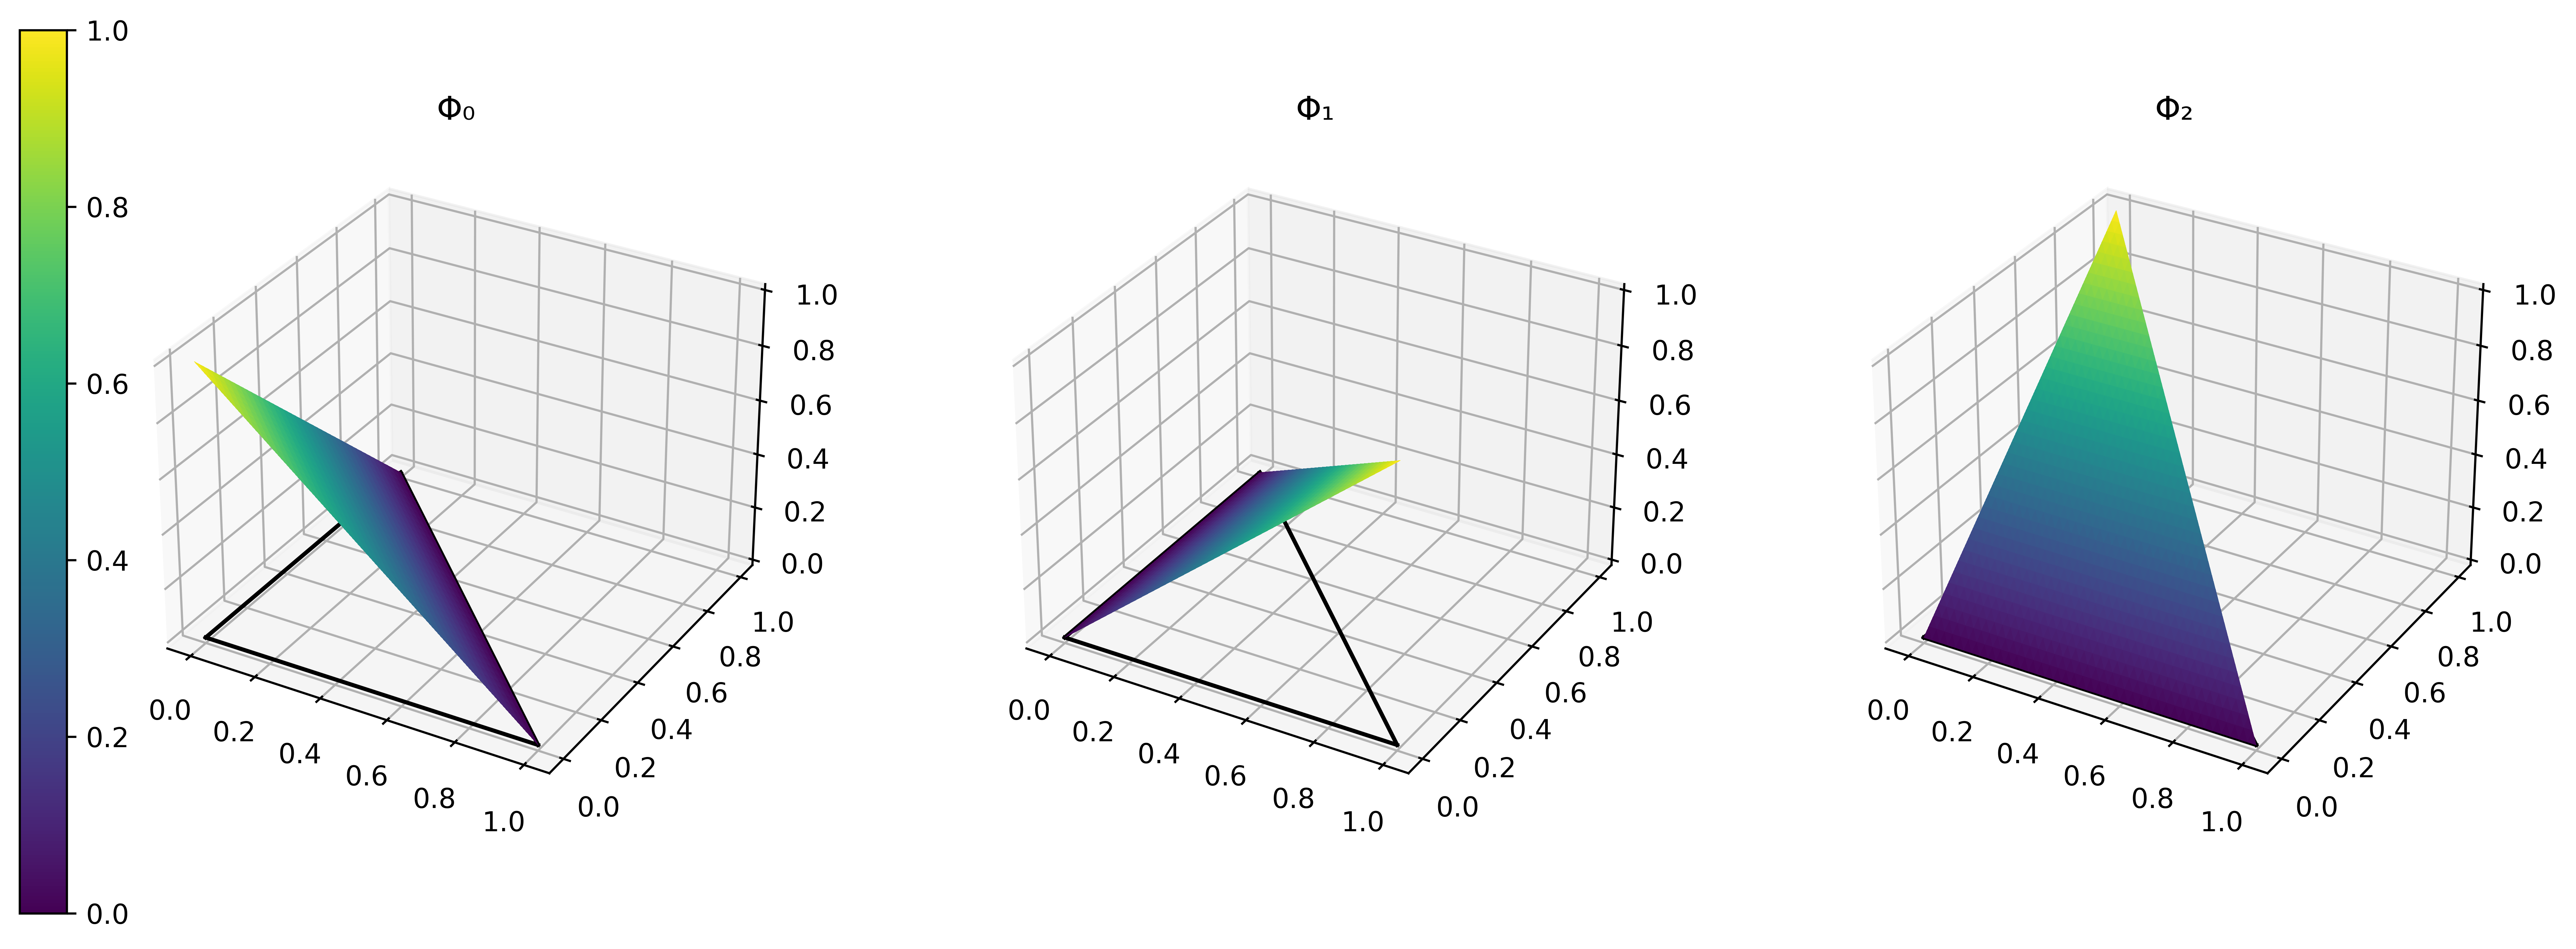
\includegraphics[width=.8\linewidth]{p1_2d_mesh_basis}
    \caption{Polynomial of degree 1 on the 2-unit-simplex}
  \end{subfigure}
  \begin{subfigure}{1.\textwidth}
    \centering
    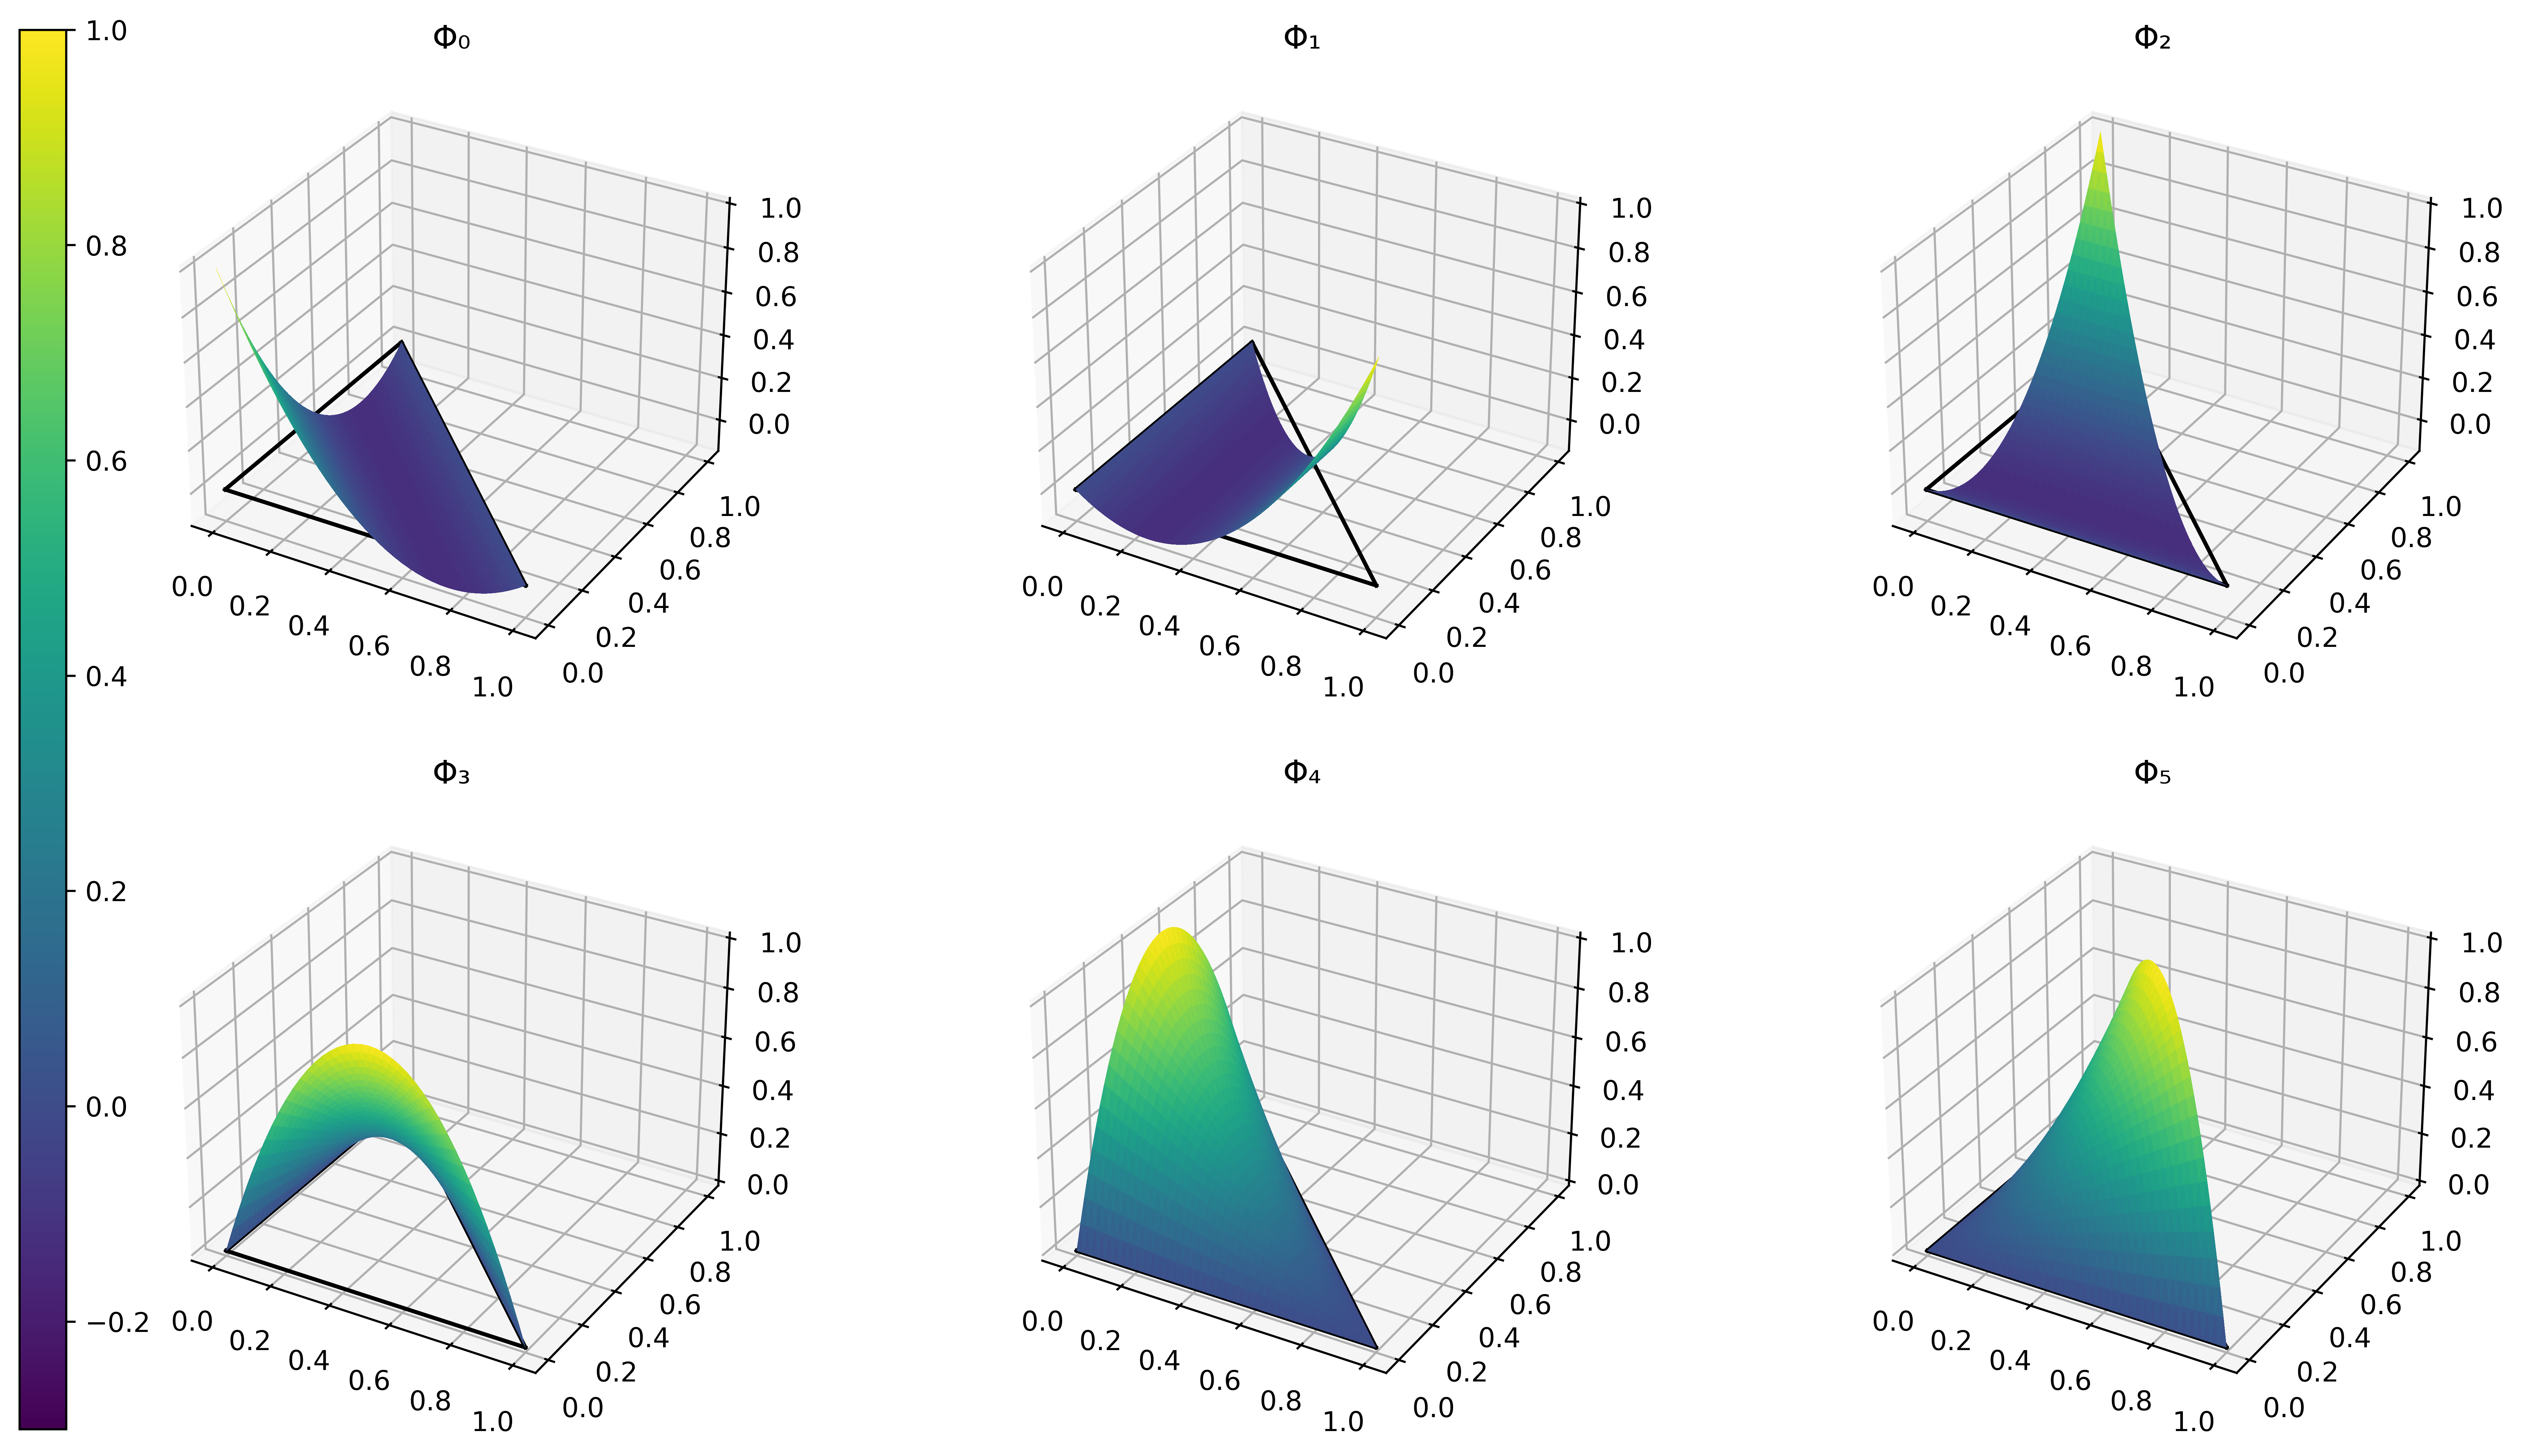
\includegraphics[width=.8\linewidth]{p2_2d_mesh_basis}
    \caption{Polynomial of degree 2 on the 2-unit-simplex}
  \end{subfigure}
  \caption{Polynomial basis on the 2d reference element}
  \label{fig:basis_2d}
\end{figure}


To compare how higher order elements perform compared to their linear counterparts,
the same numerical experiments as above will be repeated with higher order elements.

The following estimate for the convergence rates of $k^{\text{th}}$ order
elements has been established during the lecture:
\begin{equation}
  \lVert u - u_h \rVert_L^2 \lesssim h^{k'} \lVert u \rVert_{H^{k'+1}}
\end{equation}
Where $k' = \operatorname{min}\left(k,m\right)$ and $m$ is the largest integer s.t. $u \in H^{m+1}$.

By using Problem \ref{eq:smooth_poisson_prob} and \ref{eq:poisson_less_smooth_prob}
again, the parameter $a$ can be adjusted easily to verify the above convergence
rate for higher order elements.


Using the problem \ref{eq:smooth_poisson_prob} with $a = 5$ we have $u \in H^k(\Omega) \forall k \in \mathbb{N}$.
Thus, a convergence rate of $ \sim h^{d+1}$ for a polynomial basis of arbitrary degree $d$ in the $L^2$ norm is expected.

This is verified on a regular grid in \ref{fig:errors_smooth_highorder}.
It can be seen, that basis functions of degree $8$ and $10$ do converge very fast.
However, they stop increasing in accuracy after just a few refinement steps which is probably due to other numerical errors
associated with bad conditioning of the Vandermonde matrix and its inverse used to evaluate the basis functions.
\begin{figure}
  \centering
  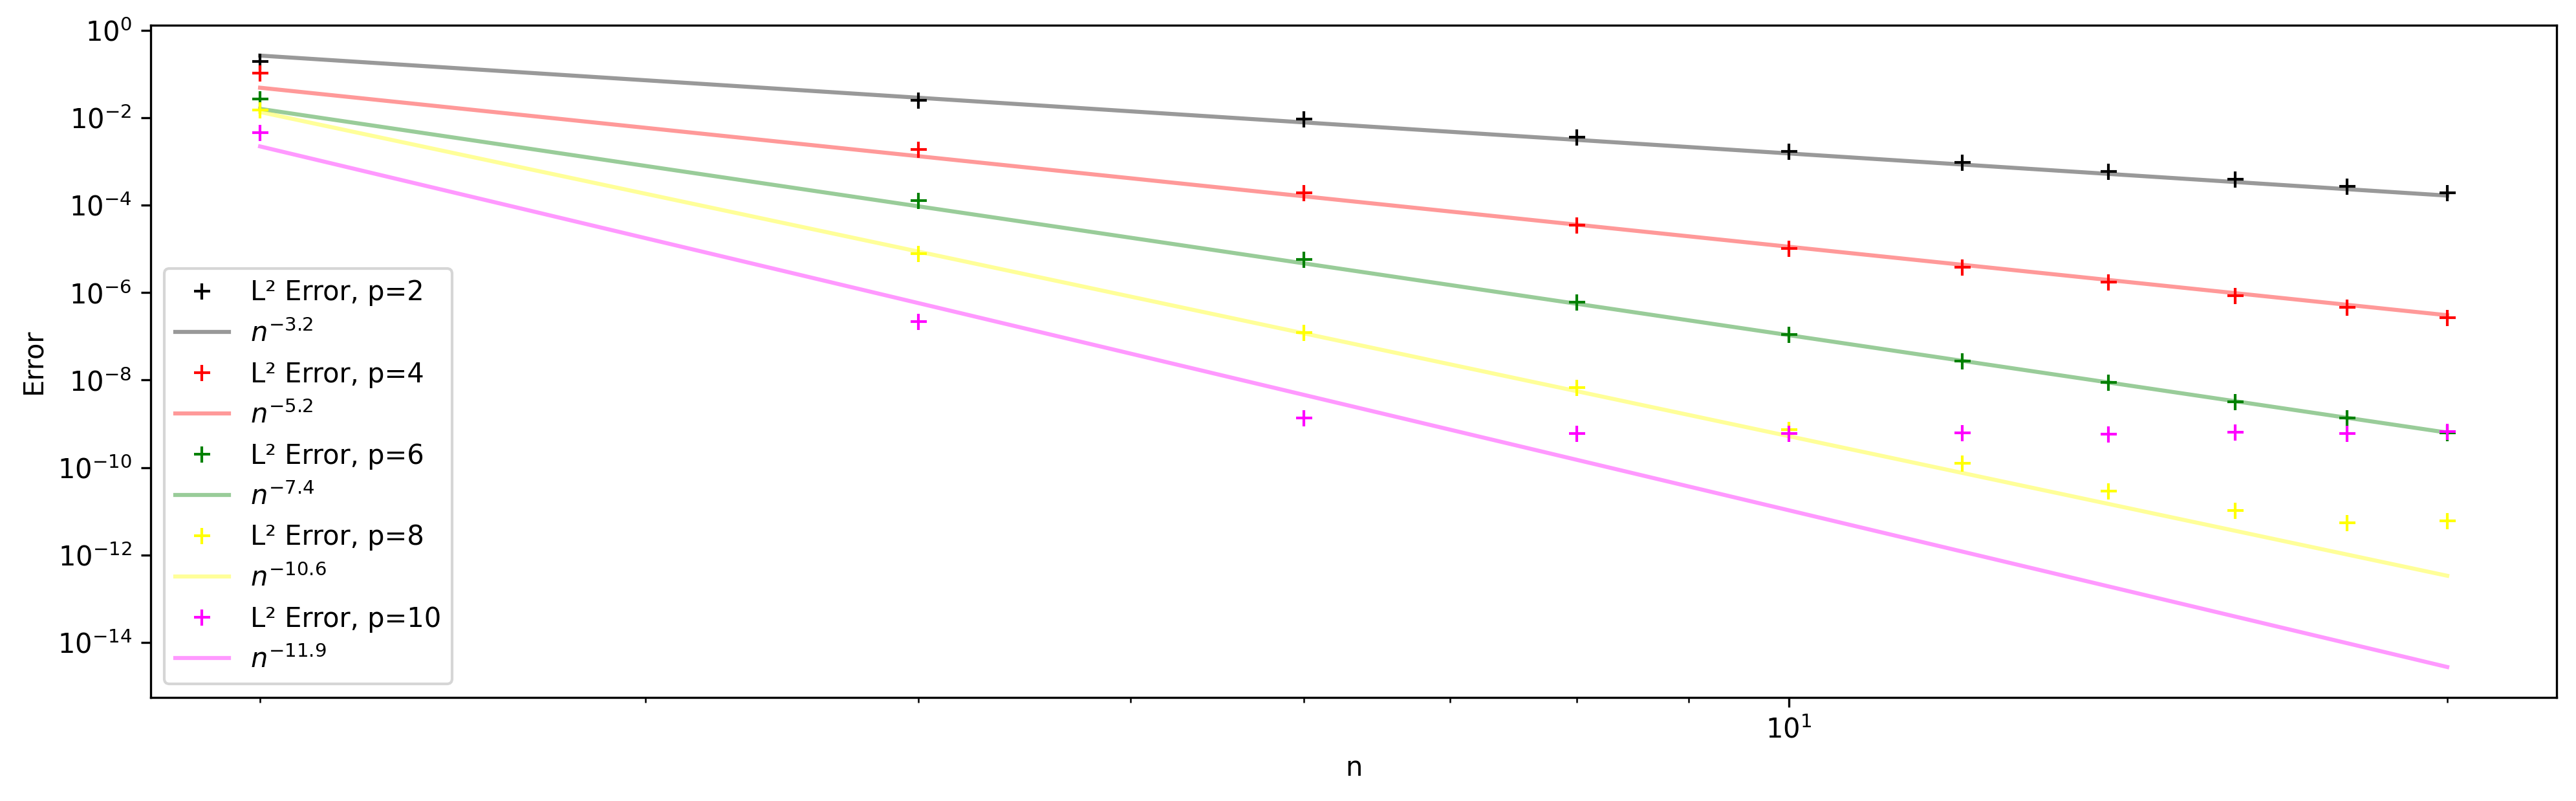
\includegraphics[width=.8\linewidth]{errors_smooth_highorder_l2}
  \caption{$L^2$ Error for Smooth Solution with Different Degree Polynomials}
  \label{fig:errors_smooth_highorder}
\end{figure}



\subsection*{Numerical Challenges With Higher Order Elements}

\end{document}
